% Tesi D.S.I. - modello preso da
% Stanford University PhD thesis style -- modifications to the report style
\documentclass[a4paper,12pt]{report}
\usepackage[a4paper]{geometry}
\usepackage{amssymb,amsmath,amsthm}
\usepackage{graphicx}
\usepackage{url}
\usepackage{hyperref}
\usepackage{epsfig}
\usepackage[italian]{babel}
\usepackage{setspace}
\usepackage{tesi}
\usepackage[utf8]{inputenc}
\usepackage{algorithmicx}
\usepackage{pythonhighlight}
\usepackage{algorithm}
\usepackage{algpseudocode}
\usepackage{enumitem}
\usepackage{tcolorbox}
\usepackage{listings}
\usepackage{tikz}
\usepackage{framed}
\usepackage{fancyvrb}
\usepackage{listings,lipsum}
\usepackage{graphicx}

\newenvironment{teor}{\begin{myteor}\sl}{\end{myteor}}
%
%
%			TITOLO: Furthest Insertion Algorithm 
%
\begin{document}
%
\includegraphics{tesiSCIENZE_TECNOLOGIE.jpg}
\title{Furthest Insertion: una nuova euristica per il TSP}
\author{Asaf COHEN}
\dept{Corso di Laurea in Informatica} 
\anno{2023-2024}
\matricola{975599}
\relatore{Prof. Giovanni RIGHINI}
%
%        \submitdate{month year in which submitted to GPO}
%		- date LaTeX'd if omitted
%	\copyrightyear{year degree conferred (next year if submitted in Dec.)}
%		- year LaTeX'd (or next year, in December) if omitted
%	\copyrighttrue or \copyrightfalse
%		- produce or don't produce a copyright page (false by default)
%	\figurespagetrue or \figurespagefalse
%		- produce or don't produce a List of Figures page
%		  (false by default)
%	\tablespagetrue or \tablespagefalse
%		- produce or don't produce a List of Tables page
%		  (false by default)
% 
%			DEDICA
%

\beforepreface

\clearpage
\null
\thispagestyle{empty}
\clearpage

\prefacesection{Ringraziamenti}
        {\hfill \Large {\sl dedicato a DA COMPLETARE\dots}}
% 
%			PREFAZIONE
%

\clearpage
\null
\thispagestyle{empty}
\clearpage

\prefacesection{Abstract}
Il Problema del Commesso Viaggiatore (TSP) rappresenta una delle sfide più interessanti e rilevanti nell'ambito dell'ottimizzazione combinatoria. Originariamente formulato negli anni '30, il TSP richiede di determinare il percorso più breve per visitare un insieme di città esattamente una volta, ritornando infine alla città di partenza. Nonostante la sua apparente semplicità concettuale, il TSP è noto per la sua complessità computazionale e la sua rilevanza pratica in una vasta gamma di settori, inclusi trasporti,  logistica, e progettazione di circuiti.

Il TSP è classificato come un problema NP-hard, il che significa che non esiste un algoritmo efficiente in grado di risolvere tutte le istanze del problema in tempo polinomiale. Di conseguenza, sono state sviluppate numerose euristiche e approcci approssimati per trovare soluzioni accettabili in un tempo ragionevole. Le euristiche sono strategie di ricerca che, pur non garantendo la soluzione ottima, sono in grado di produrre risultati soddisfacenti entro limiti temporali praticabili.

In questa tesi, esploreremo una specifica euristica per il TSP chiamata Furthest Insertion: l'obiettivo principale sarà quello di presentare, analizzare e valutare l'efficacia di questa euristica attraverso run su istanze presenti su TSP-LIB e confronti con altre tecniche note.

La scelta di concentrarsi su un'euristica per il TSP è motivata dalla necessità di affrontare problemi di dimensioni reali in contesti applicativi. Mentre le soluzioni esatte sono desiderabili per la loro precisione, spesso richiedono una potenza di calcolo eccessiva per problemi di grandi dimensioni. Le euristiche offrono un compromesso utile tra precisione e efficienza, consentendo di ottenere soluzioni praticabili che possono guidare decisioni reali.

Questa tesi sarà strutturata nel seguente modo: innanzitutto, forniremo una panoramica del TSP e della sua formulazione matematica. Successivamente, esamineremo le principali categorie di approcci risolutivi, concentrandoci in particolare sulle euristiche basate su inserzione. Presenteremo quindi la nuova euristica Furthest Insertion discutendo la sua implementazione e le scelte progettuali adottate. Infine, concluderemo con un'analisi dei risultati ottenuti, identificando i punti di forza e le limitazioni della nuova euristica.

\afterpreface
% 
% 
%			CAPITOLO 1: Introduzione
\chapter{Il Problema del Commesso Viaggiatore}
Il Problema del Commesso Viaggiatore (TSP) è una delle sfide più emblematiche e studiate nell'ambito della ricerca operativa e dell'ottimizzazione combinatoria. Originariamente formulato negli anni '30 da Karl Menger \cite{Menger}, il TSP richiede di determinare il percorso più breve per visitare un insieme di città esattamente una volta, tornando infine alla città di partenza. Nonostante la sua semplice descrizione concettuale, il TSP è noto per la sua complessità computazionale e la sua rilevanza pratica in una vasta gamma di settori.

Le applicazioni del TSP sono diffuse e impattano direttamente su molte attività quotidiane. Ad esempio, nel settore della logistica e della gestione delle catene di distribuzione, il TSP è utilizzato per ottimizzare le rotte dei veicoli di consegna, minimizzando i costi di carburante e il tempo impiegato. In ambito produttivo, il TSP viene impiegato per pianificare i percorsi di ispezione delle fabbriche o per ottimizzare il flusso di lavoro all'interno di un'azienda. Anche nei sistemi di navigazione satellitare e nelle applicazioni GPS, il TSP è alla base dell'ottimizzazione dei percorsi per ridurre il tempo di viaggio.

Storicamente, il TSP ha attratto l'attenzione di numerosi matematici e informatici in quanto è un problema semplice da formulare ma complesso da "risolvere". Il problema è stato formalizzato e reso noto grazie al lavoro di Hassler Whitney nel 1952\footnote[1]{https://www.math.uwaterloo.ca/tsp/uk/history.html} e successivamente nel 1954 da Merrill Flood. La dimostrazione della sua appartenenza alla classe di complessità NP-hard è stata fondamentale per stimolare lo sviluppo di tecniche approssimate e euristiche. Le sfide legate al TSP sono principalmente dovute alla sua natura combinatoria: per n città, il numero di possibili percorsi da valutare cresce in modo esponenziale con n, rendendo impraticabile un'analisi esaustiva per istanze di grandi dimensioni. Questa complessità ha spinto alla ricerca di approcci efficienti, come le euristiche, che non garantiscono la soluzione ottimale ma forniscono soluzioni accettabili in tempi ragionevoli.

\section{Il Problema del commesso viaggiatore}
Il problema del commesso viaggiatore (TSP) può essere sintetizzato molto semplicemente con la seguente domanda: "Date n città, qual è il percorso più breve che inizia e termina con la stessa città?". Il problema quindi presenta le caratteristiche tipiche di un problema su un grafo, dove il grafo è composto da $n$ vertici (le città) e dove gli archi indicano le distanze euclidee tra le città. La formulazione classica del TSP può essere descritta matematicamente attraverso la programmazione intera lineare. La seguente formulazione fa riferimento alla formulazione MTZ (Miller-Tucker-Zemlin) e alla formulazione DFJ (Dantzig-Fulkerson-Johnson) \cite{TSP formulation}.
\section{Formulazione del problema}
\textbf{Dati}: Consideriamo un insieme di $n$ città, ogni città $i$ (per $i = 1, 2, ..., n$) rappresenta un punto nello spazio euclideo, ogni città quindi ha coordinate $(x_i, y_i)$. Definiamo la matrice $c$, dove $c_{ij}$ indica la distanza euclidea tra le due città $i$ e $j$.
\\[1\baselineskip]
\textbf{Variabili}: La variabile $x_{ij}$ è una variabile binaria, quindi: $$ x_{ij} \in \{0, 1\} \qquad \forall i, j = 1, 2, 3, ..., n $$ La variabile $x$ assume valore 0 se l'arco che collega la città $i$ e $j$ non fa parte del path, 1 se ne fa parte.
\\[1\baselineskip] \textbf{Vincoli}: I vincoli sono i seguenti:
\begin{enumerate}
        \item Per ogni città $i$ deve essere presente un solo arco uscente corrispondente nel tour, quindi la somma delle variabili $x_{ij}$ deve essere uguale a 1. $$\sum_{j = 1}^{n} x_{ij} = 1 \qquad \forall i = 1, 2, 3, ..., n$$
        \item Per ogni città $j$ deve essere presente un solo arco entrante corrispondente nel tour, quindi la somma delle variabili $x_{ij}$ deve essere uguale a 1. $$\sum_{i = 1}^{n} x_{ij} = 1 \qquad \forall j = 1, 2, 3, ..., n$$
        \item Non devono essere presenti cicli all'interno del tour, quindi deve valere: $$ \sum_{i \in Q}{\sum_{j \in Q}{x_{ij} \le |Q| - 1}} \qquad \forall Q \subsetneq \{2, 3, ..., n\} $$
\end{enumerate}
\textbf{Funzione Obiettivo}: Si vuole minimizzare il costo totale del tour, quindi:
$$min \sum_{i = 1}^{n} \sum_{j = 1}^{n} c_{ij} x_{ij}$$
La seguente formulazione permette quindi di identificare la soluzione ottima.
\newline \null \newline È stato dimostrato che TSP è un problema NP-hard \cite{TSP NP Completezza}, questo implica che attualmente non sono noti algoritmi con complessità polinomiale che risolvono il problema. Se esistesse un algoritmo con complessità polinomiale che risolve il TSP allora si potrebbe dimostrare che vale P = NP e quindi si risolverebbe uno dei più grandi problemi aperti nella teoria della complessità computazionale. 

\section{Metodi esatti per il TSP}
Esistono vari approcci nella ricerca della soluzione ottima \cite{Analysis of Brute Force}. Un primo approccio "naive" per il problema può essere l'approccio brute-force: consiste nell'enumerare tutti i possibili percorsi e successivamente selezionare il migliore. In questo caso è necessario analizzare $n!$ possibili percorsi (nel peggiore dei casi), per questo motivo tentare di risolvere una istanza TSP con un approccio brute-force implica una complessità computazionale pari a $O(n!)$ e quindi un tempo che risulta rapidamente inaccettabile. Di seguito una tabella che illustra il numero di percorsi da valutare con un approccio basato su ricerca esaustiva al variare del numero n.



\begin{center}
        \begin{tabular}{|c|c|}
                \hline
                \textbf{Numero città} & \textbf{Numero percorsi possibili} \\ % Intestazione in grassetto
                \hline % Linea orizzontale sopra della tabella
                4 & 24 \\
                \hline
                5 & 120 \\
                \hline
                6 & 720 \\
                \hline
                7 & 5,040 \\
                \hline
                8 & 40,320 \\
                \hline
                9 & 362,880 \\
                \hline
                10 & 3,628,800 \\
                \hline
                11 & 39,916,800 \\
                \hline
                12 & 479,001,600 \\
                \hline
                13 & 6,227,020,800 \\
                \hline
                14 & 87,178,291,200 \\
                \hline
                15 & 1,307,674,368,000 \\
                \hline
                16 & 20,922,789,888,000 \\
                \hline
                17 & 355,687,428,096,000 \\
                \hline
                18 & 6,402,373,705,728,000 \\
                \hline
                19 & 121,645,100,408,832,000 \\
                \hline
                20 & 2,432,902,008,176,640,000 \\
                \hline
                21 & 51,090,942,171,709,440,000 \\
                \hline
                22 & 1,124,000,727,777,607,680,000 \\
                \hline
                23 & 25,852,016,738,884,976,640,000 \\
                \hline
                24 & 620,448,401,733,239,439,360,000 \\
                \hline
                25 & 15,511,210,043,330,985,984,000,000 \\
                \hline
        \end{tabular}
        \newline
\end{center}
Si può notare come il numero cresce molto rapidamente, anche con istanze relativamente piccole (ad esempio 20 città). Questo approccio risulta quindi inutilizzabile nei problemi reali dove può essere necessario analizzare istanze con migliaia di città.
\newline \null \newline Esistono altri algoritmi esatti i quali consentono di ridurre il numero di possibili soluzioni (percorsi) da analizzare, ad esempio approcci Branch and Bound \cite{Branch and Bound}. La complessità computazionale nel caso peggiore resta esponenziale in quanto può essere necessario analizzare un numero esponenziale di percorsi e quindi non applicabile su problemi reali.
\newline \null \newline 
Oltre all'approccio brute force, esistono in letteratura diversi algoritmi \textbf{branch-and-bound}\footnote[1]{https://www.math.cmu.edu/~bkell/21257-2014f/tsp.pdf}\footnote[2]{https://apps.dtic.mil/sti/tr/pdf/ADA142318.pdf} che consentono di risolvere in problema in modo più efficiente. L'idea alla base consiste nel suddividere il problema originario in sottoproblemi (più semplici) i quali possono essere a loro volta scomposti in ulteriori sottoproblemi. Il termine "bound" indica il fatto che per ogni sottoproblema viene calcolato il limite inferiore $L_i$ (quindi la soluzione ottima non sarà mai migliore di questo limite inferiore) e si tiene conto della soluzione migliore trovata fino a quel punto $U$: quando $L_i$ è "peggiore" di $U$ allora è possibile scartare a priori l'intero sottoproblema in quanto è già stata trovata una soluzione migliore del limite inferiore del sottoproblema (questo processo prende il nome di "pruning"). Il termine "branch" invece fa riferimento al fatto che i sottoproblemi vengono a loro volta divisi in ulteriori sottoproblemi (come visto prima), l'algoritmo branch-and-bound procede esplorando l'albero dei sottoproblemi generati (detto anche albero branch-and-bound) e scartando i sottoproblemi (pruning) con il criterio visto prima. I vari algoritmi differiscono in base al criterio di branching e di esplorazione dell'albero branch-and-bound. \newline \null \newline
Lo stato dell'arte degli algoritmi esatti per il TSP non sono i generici branch-and-bound ma sono algoritmi \textbf{branch-and-cut}\cite{Branch and Cut}: Branch and Cut è un metodo di ottimizzazione combinatoria simile al branch and bound, ma con alcune differenze fondamentali. Entrambi gli algoritmi mirano a trovare la soluzione ottimale per un problema complesso, dividendolo in sottoproblemi più piccoli e scartando (pruning) i sottoproblemi che in ogni caso non possono portare ad una soluzione parziale migliore di quella già nota. Tuttavia, l'algoritmo Branch and Cut si distingue per l'utilizzo di vincoli di taglio (cutting planes). Di seguito viene illustrato un generico algoritmo branch-and-cut:
\newlist{legal}{enumerate}{10}
\setlist[legal]{label*=\arabic*.}

\begin{tcolorbox}[colframe=black,colback=white,boxrule=0.5pt, sharp corners]
\begin{legal}
  \item Aggiungi il problema iniziale $ILP$ alla lista dei problemi attivi $L$.
  \item Sia $x^* = null$ e $v^* = -\infty$
  \item Finché $L$ non è vuota:
  \begin{legal}
    \item Seleziona e rimuovi un problema da L
    \item Risolvi il rilassamento continuo di L
    \item Se il problema è inammissibile torna al punto 3 (ciclo while). Altrimenti sia $x$ la soluzione trovata e $v$ il valore della funzione obiettivo.
    \item Se $v \leq v^*$ torna al punto 3
    \item Se $x$ è intero, aggiorna $v^* \leftarrow v$, $x^* \leftarrow x$ e torna al punto 3.
    \item Cerca dei piani di taglio che sono violati da $x$, se sono presenti aggiungili al rilassamento continuo di ILP e torna al punto 3.2
    \item Dividi il problema in sottoproblemi, aggiungi i sottoproblemi alla lista dei problemi attivi $L$, torna al punto 3.
  \end{legal}
  \item Restituisci $x^*$


\end{legal}
\end{tcolorbox}
\hfill \break
Come già detto in precedenza, questo approccio è attualmente lo stato dell'arte per risolvere il TSP all'ottimo. In letteratura esistono varie implementazioni di algoritmi branch-and-cut per il TSP\cite{Branch and Cut Algoritmhs}, sono presenti anche all'interno di risolutori MILP come ad esempio CPLEX. Questo approccio risulta migliore rispetto all'approccio brute-force, ma resta comunque non applicabile su istanze TSP con migliaia di città.

\chapter{Euristiche per il TSP}
Come discusso nel capitolo 2, i metodi esatti consentono di ottenere soluzioni ottime per il problema del TSP, ma il tempo per ottenere queste soluzioni aumenta esponenzialmente all'aumentare del numero di città presenti nell'istanza. Per affrontare il TSP, sono stati sviluppati numerosi approcci euristici, ovvero metodi che, pur non garantendo la soluzione ottimale, offrono soluzioni di buona qualità in tempi ragionevoli. Le euristiche sono fondamentali per applicazioni pratiche dove la rapidità di calcolo è essenziale. In questo capitolo esploreremo diverse tecniche euristiche, come le euristiche costruttive, che costruiscono una soluzione passo dopo passo a partire da una soluzione parziale, vedremo in particolare sulle euristiche basate su inserzione (Furthest Insertion fa parte di questa categoria) e poi "improvement euristics" ovvero le euristiche basate su meccanismi che consentono di "migliorare" la soluzione parziale trovata modificando il tour.
\section{Nearest Neighbor} \label{sec:NN}
Nearest Neighbor è probabilmente l'euristica costruttiva più semplice per il TSP: si costruisce il tour selezionando sempre la città più vicina all'ultima appena aggiunta al tour. Appartiene alla categoria delle euristiche costruttive in quanto aggiunge via via nuove città al tour (soluzione parziale) senza modificare il tour costruito fino a quel punto. L'algoritmo è il seguente:

\setlist[legal]{label*=\arabic*.}
\begin{tcolorbox}[colframe=black,colback=white,boxrule=0.5pt, sharp corners]
\begin{legal}
  \item Seleziona un nodo arbitrario j, sia l = j e L = $\{1, 2, ..., n\} \setminus \{j\}$.
  \item Finché $L \neq \emptyset$:
  \begin{legal}
    \item Sia $j \in L$ tale che $c_{lj} = min\{c_{li} \  | \  i \in L\}$.
    \item Connetti l a j e rimuovi j da L, quindi $ L = L \setminus \{j\} $.
  \end{legal}
  \item Connetti l al primo nodo (era stato selezionato al punto 1) per formare un tour.
\end{legal}
\end{tcolorbox}
\hfill \break
Nearest Neighbor è una euristica con complessità temporale pari a $O(n^2)$ in quanto per ogni nodo nel tour (quindi n volte) è necessario cercare tra i restanti nodi, qual è il più vicino (al massimo n volte).

\section{Euristiche basate su Inserzione}
Le euristiche basate su inserzione appartengono alla categoria delle euristiche costruttive ma a differenza di Nearest Neighbor la soluzione viene costruita in un modo differente: si inizia da un piccolo tour (che include 2 o 1 città) il quale viene via via esteso includendo i nodi (città) non ancora aggiunti al tour. In questo tipo di euristiche la differenza fondamentale che le distingue sarà il criterio con il quale si aggiungono nuove città al tour e dove queste città devono essere inserite nel tour. Una qualunque euristica basata su inserzione quindi presenta la seguente struttura:

\setlist[legal]{label*=\arabic*.}
\begin{tcolorbox}[colframe=black,colback=white,boxrule=0.5pt, sharp corners]
\begin{legal}
  \item Seleziona una città o due città arbitrarie come tour iniziale $T$. Sia $L$ l'insieme delle città che sono fuori dal tour, quindi: $L = \{1, 2, ..., n\} \setminus T$.
  \item Finché $L \neq \emptyset$:
  \begin{legal}
    \item Seleziona un nodo $j \in L$ secondo un certo criterio.
    \item Inserisci $j$ nel tour in una determinata posizione.
    \item Rimuovi $j$ da L, quindi $L = L \setminus \{j\}$.
  \end{legal}
\end{legal}
\end{tcolorbox}
\hfill \break
Questo schema permette di ottenere un ciclo Hamiltoniano e quindi un percorso valido per il problema del TSP. Le varie euristiche andranno a definire un criterio di scelta del nodo j (punto 2.1) e un criterio di scelta della posizione di inserzione (punto 2.2).

\subsection{Nearest Insertion} \label{ssec:NI}
Nearest Insertion seleziona come nodo da inserire nel tour il nodo più vicino ad un qualunque nodo già inserito nel tour e lo inserisce nella posizione che minimizza il costo di inserimento. Di seguito l'algoritmo:

\setlist[legal]{label*=\arabic*.}
\begin{tcolorbox}[colframe=black,colback=white,boxrule=0.5pt, sharp corners]
  \begin{legal}
    \item Sia $T$ il tour iniziale definito dalla coppia delle città più lontane. Sia $L$ l'insieme delle città fuori dal tour, quindi: $L = \{1, 2, ..., n\} \setminus T$.
    \item Finché $L \neq \emptyset$:
    \begin{legal}
      \item Sia $d_{min}(v)$ la distanza minima tra il nodo $v$ e il tour $T$, ovvero $d_{min}(v) = min\{c_{vt} | t \in T \}$. Seleziona il nodo $r \not \in T$ in modo da \underline{minimizzare} $d_{min}(r)$.
      \item Determina la posizione ottima di inserzione $(a, b)$ in modo da \underline{minimizzare} il costo di inserimento $c_{ar} + c_{rb} - c_{ab}$, inserisci $r$ tra $(a, b)$
      \item Rimuovi $r$ da L, quindi $L = L \setminus \{r\}$.
    \end{legal}
  \end{legal}
  \end{tcolorbox}
\hfill \break Nearest Insertion ha complessità computazionale pari a $O(n^2)$ in quanto ogni nodo (n iterazioni) deve essere inserito nel modo migliore possibile nel tour (fino a n iterazioni).

\subsection{Cheapest Insertion} \label{ssec:CI}
Cheapest Insertion opera in modo diverso da Nearest Insertion: il criterio di selezione non è più il nodo più vicino al tour, ma diventa il nodo che produce il minor aumento del costo del tour se inserito (quindi minimizza il costo di inserzione). Una volta selezionato, il nodo viene inserito nel modo migliore possibile, quindi minimizzando il costo di inserimento. Di seguito l'algoritmo:

\setlist[legal]{label*=\arabic*.}
\begin{tcolorbox}[colframe=black,colback=white,boxrule=0.5pt, sharp corners]
  \begin{legal}
    \item Sia $T$ il tour iniziale definito dalla coppia delle città più lontane. Sia $L$ l'insieme delle città fuori dal tour, quindi: $L = \{1, 2, ..., n\} \setminus T$.
    \item Finché $L \neq \emptyset$:
    \begin{legal}
      \item $\forall v \not \in T$, determina il punto di inserzione $P(v)$ (ovvero l'arco $(a, b) \in T$) in modo da \underline{minimizzare} $c_{av} + c_{vb} - c_{ab}$, sia $C(v)$ il costo di inserimento del nodo $v$ nel punto di inserzione trovato.
      \item Tra tutti i nodi fuori dal tour, seleziona il nodo $r$ in modo da \underline{minimizzare} $C(r)$
      \item Inserisci il nodo $r$ nel punto di inserzione $P(r)$ trovato prima
      \item Rimuovi $r$ da L, quindi $L = L \setminus \{r\}$.
    \end{legal}
  \end{legal}
  \end{tcolorbox}
\hfill \break La complessità computazionale di questa euristica verrà discussa nella sezione nel capitolo delle implementazioni in quanto verranno presentate più versioni (con complessità differenti).

\subsection{Farthest Insertion} \label{ssec:FaI}
Farthest Insertion opera in analogo a Nearest Insertion in quanto il criterio di selezione del nodo da inserire è basato sulla distanza dal tour, ma differenza di Nearest Insertion però viene scelto il nodo più lontano dal tour al posto del più vicino. Il passo di inserzione avviene invece allo stesso modo rispetto a Nearest Insertion: viene quindi scelta la posizione che minimizza il costo di inserzione. Vediamo l'algoritmo:

\setlist[legal]{label*=\arabic*.}
\begin{tcolorbox}[colframe=black,colback=white,boxrule=0.5pt, sharp corners]
\begin{legal}
  \item Sia $T$ il tour iniziale definito dalla coppia delle città più lontane. Sia $L$ l'insieme delle città fuori dal tour, quindi: $L = \{1, 2, ..., n\} \setminus T$.
  \item Finché $L \neq \emptyset$:
  \begin{legal}
    \item Sia $d_{min}(v)$ la distanza minima tra il nodo $v$ e il tour $T$, ovvero $d_{min}(v) = min\{c_{vt} | t \in T \}$. Seleziona il nodo $r \not \in T$ in modo da \underline{massimizzare} $d_{min}(r)$.
    \item Determina la posizione ottima di inserzione $(a, b)$ in modo da \underline{minimizzare} il costo di inserimento $c_{ar} + c_{rb} - c_{ab}$, inserisci $r$ tra $(a, b)$
    \item Rimuovi $r$ da L, quindi $L = L \setminus \{r\}$.
  \end{legal}
\end{legal}
\end{tcolorbox}
\hfill \break Farthest Insertion ha complessità computazionale pari a $O(n^2)$ in modo del tutto analogo a Nearest Insertion.

\subsection{Furthest Insertion} \label{ssec:FuI}
L'obbiettivo della tesi consiste nel proporre un nuovo algoritmo chiamato Furthest Insertion: allo stesso modo in cui Farthest Insertion opera in modo analogo a Nearest Insertion, Furthest Insertion opera in modo analogo a Cheapest Insertion. Il passo di selezione consiste nel selezionare il nodo che massimizza il costo di inserzione, in fase di inserimento però il nodo viene inserito in modo da minimizzare il costo di inserimento. Di seguito l'algoritmo:

\setlist[legal]{label*=\arabic*.}
\begin{tcolorbox}[colframe=black,colback=white,boxrule=0.5pt, sharp corners]
\begin{legal}
  \item Sia $T$ il tour iniziale definito dalla coppia delle città più lontane. Sia $L$ l'insieme delle città fuori dal tour, quindi: $L = \{1, 2, ..., n\} \setminus T$.
  \item Finché $L \neq \emptyset$:
  \begin{legal}
    \item $\forall v \not \in T$, determina il punto di inserzione $P(v)$ (ovvero l'arco $(a, b) \in T$) in modo da \underline{minimizzare} $c_{av} + c_{vb} - c_{ab}$, sia $C(v)$ il costo di inserimento del nodo $v$ nel punto di inserzione trovato.
    \item Tra tutti i nodi fuori dal tour, seleziona il nodo $r$ in modo da \underline{massimizzare} $C(r)$
    \item Inserisci il nodo $r$ nel punto di inserzione $P(r)$ trovato prima
    \item Rimuovi $r$ da L, quindi $L = L \setminus \{r\}$.
  \end{legal}
\end{legal}
\end{tcolorbox}
\hfill \break La complessità computazionale di questa euristica verrà discussa nella sezione nel capitolo delle implementazioni (come per Cheapest Insertion) in quanto verranno presentate più versioni (con complessità differenti).

\subsection{Random Insertion} \label{ssec:RI}
Random Insertion seleziona casualmente il nodo da inserire nel tour, successivamente però sceglie il punto di inserimento in modo da minimizzare il costo di inserimento (esattamente come per Nearest Insertion). Di seguito l'algoritmo:

\setlist[legal]{label*=\arabic*.}
\begin{tcolorbox}[colframe=black,colback=white,boxrule=0.5pt, sharp corners]
\begin{legal}
  \item Sia $T$ il tour iniziale definito da una città casuale. Sia $L$ l'insieme delle città fuori dal tour, quindi: $L = \{1, 2, ..., n\} \setminus T$.
  \item Finché $L \neq \emptyset$:
  \begin{legal}
    \item Seleziona un nodo $r \in L$ casualmente.
    \item Seleziona l'arco $(i, j)$ in $T$ tale che $c_{ir} + c_{rj} - c_{ij}$ risulti \underline{minimo}.
    \item Inserisci $r$ tra $i$ e $j$.  
    \item Rimuovi $r$ da L, quindi $L = L \setminus \{r\}$.
  \end{legal}
\end{legal}
\end{tcolorbox}
\hfill \break Random Insertion ha complessità computazionale pari a $O(n^2)$ in quanto n volte viene selezionato un nodo casuale, dopodiché è necessario iterare n volte alla ricerca della posizione migliore dove inserire il nodo.

\section{Ricerca Locale}
Le euristiche basate su ricerca locale\cite{Local Search} sono euristiche che implementano un meccanismo che consente di migliorare un tour (anche parziale), il meccanismo può ad esempio scambiare due nodi nel tour (vedremo nel dettaglio una euristica in particolare), rimuovere un nodo e inserirlo in un punto del tour migliore oppure implementare meccanismi più sofisticati.

\subsection{Node Insertion}
Questa euristica permette di migliorare un tour rimuovendo un nodo e inserendolo nel tour nel modo migliore possibile. Di seguito la procedura:

\setlist[legal]{label*=\arabic*.}
\begin{tcolorbox}[colframe=black,colback=white,boxrule=0.5pt, sharp corners]
\begin{legal}
  \item Sia $T$ il tour (anche parziale).
  \item Ripeti finché il tour $T$ resta invariato:
  \begin{legal}
    \item Per ogni nodo $i = 1, 2, ..., n$: è possibile ridurre la lunghezza del tour rimuovendo il nodo i da una posizione $p_1$ e inserendo il nodo $i$ in un'altra posizione $p_2$? Se si, aggiorna $T$ spostando il nodo $i$ da $p_1$ a $p_2$.
  \end{legal}
\end{legal}
\end{tcolorbox}
\hfill \break
La procedura richiede tempo $O(n^2)$ in quanto per ogni nodo (n volte) è necessario ispezionare il possibile scambio di posizione (n volte).

\subsection{Edge Insertion}
In modo analogo a Node Insertion, questa euristica permette di migliorare un tour rimuovendo un arco (a differenza del nodo di prima) e inserendolo nel tour nel modo migliore possibile. Di seguito la procedura:

\setlist[legal]{label*=\arabic*.}
\begin{tcolorbox}[colframe=black,colback=white,boxrule=0.5pt, sharp corners]
\begin{legal}
  \item Sia $T$ il tour (anche parziale).
  \item Ripeti finché il tour $T$ resta invariato:
  \begin{legal}
    \item Per ogni nodo $i = 1, 2, ..., n$, considera l'arco che collega $i$ con il nodo successivo nel tour, sia $(i, j)$ questo arco: è possibile ridurre la lunghezza del tour rimuovendo l'arco $(i, j)$ da una posizione $p_1$ e inserendo $(i, j)$ in un'altra posizione $p_2$? Se si, aggiorna $T$ spostando l'arco da $p_1$ a $p_2$.
  \end{legal}
\end{legal}
\end{tcolorbox}
\hfill \break
La procedura richiede tempo $O(n^2)$ in modo del tutto analogo a Node Insertion.

\subsection{Euristica 2-Opt}
L'algoritmo 2-Opt\cite{2OPT} consente di eliminare due archi e di riconnetterli in un modo diverso, andando quindi a modificare il tour. Questa euristica deriva dall'osservazione empirica per cui due archi che si incrociano possono essere sempre riorganizzati in modo da non incrociarsi e questo produce sempre una riduzione della lunghezza totale del tour. La procedura consente di ridurre la lunghezza del tour riorganizzando una coppia di archi anche quando non si incrociano. Si nota che è sempre possibile ricombinarli in un unico modo diverso. Di seguito la procedura 2-Opt:

\setlist[legal]{label*=\arabic*.}
\begin{tcolorbox}[colframe=black,colback=white,boxrule=0.5pt, sharp corners]
\begin{legal}
  \item Sia $T$ il tour (anche parziale).
  \item Ripeti finché il tour $T$ resta invariato:
  \begin{legal}
    \item Per ogni nodo $i = 1, 2, ..., n$, considera tutti gli scambi 2-Opt possibili con l'arco $(i, j)$ dove $j$ è il nodo successivo ad $i$ nel tour. Se è possibile ridurre la lunghezza del tour applicando lo scambio 2-Opt, aggiorna T.
  \end{legal}
\end{legal}
\end{tcolorbox}
\hfill \break

\subsection{Euristica 3-Opt}
L'euristica 3-Opt è un'estensione dell'euristica vista precedentemente: al posto di eliminare due archi per ricombinarli in modo diverso, in questa euristica sono 3 gli archi che l'euristica rimuove e ricombina in modo diverso. A differenza di 2-Opt sono 8 i modi diversi in cui possono essere ricombinati questi archi\footnote{http://tsp-basics.blogspot.com/2017/03/3-opt-move.html} (includendo anche la configurazione in cui gli archi restano immutati). Vediamo l'algoritmo:

\setlist[legal]{label*=\arabic*.}
\begin{tcolorbox}[colframe=black,colback=white,boxrule=0.5pt, sharp corners]
  \begin{legal}
    \item Sia $T$ il tour.
    \item Per ogni nodo $i \in V$, sia $N(i)$ un insieme di nodi.
    \item Ripeti finché il tour $T$ resta invariato:
    \begin{legal}
      \item Per ogni nodo $i = 1, 2, ..., n$: considera tutti gli scambi 3-Opt possibili che includa $i$ e un nodo nell'insieme $N(i)$. Se è possibile ridurre la lunghezza del tour in questo modo, aggiorna T.
    \end{legal}
  \end{legal}
\end{tcolorbox}
\hfill \break
La scelta di ridurre l'insieme dei nodi $V$ a $N(i)$ è necessario in quanto analizzare tutti i possibili scambi che includano 3 nodi implica un tempo $O(n^3)$. L'insieme $N(i)$ può essere generato a partire a partire dal nodo $i$ ad esempio selezionando i 10 nodi più vicini ad $i$.
      
\subsection{Euristica Lin-Kernighan}
L'algoritmo Lin-Kernighan (LK)\cite{LK} è una delle migliori euristiche per risolvere il TSP. Appartiene alla classe degli algoritmi di ricerca locale, che prendono come input un tour (ciclo hamiltoniano) e tentano di migliorarlo cercando nella sua vicinanza un tour più corto, e una volta trovato ripetono il processo da quel nuovo tour, fino a incontrare un minimo locale.
L'algoritmo LK è stato sviluppato da Serge Lin e Brian Kernighan nel 1971 ed è stato dimostrato essere molto efficace per risolvere istanze di TSP di medie e grandi dimensioni. È spesso utilizzato come componente di algoritmi ibridi per il TSP, combinandolo con altre tecniche di ricerca per ottenere risultati ancora migliori. Di seguito una descrizione ad alto livello dell'algoritmo:
\setlist[legal]{label*=\arabic*.}
\begin{tcolorbox}[colframe=black,colback=white,boxrule=0.5pt, sharp corners]
  \begin{legal}
    \item Sia $T$ il tour iniziale, può essere generato casualmente oppure tramite altre euristiche come Nearest Neighbor. Sia $S$ la soluzione migliore fino a questo momento.
    \item Ripeti finché il tour $T$ resta invariato (e quindi è stato trovato un minimo locale):
    \begin{legal}
      \item Applica l'algoritmo k-Opt. Inizialmente $k$ deve essere un valore piccolo (2 o 3), aumenta man mano il valore $k$.
    \end{legal}
    \item Una volta trovato un minimo locale, se è migliore di $S$ allora aggiorna $S$. Torna al punto 1 generando un tour diverso da quello di partenza, oppure l'algoritmo termina e S è la soluzione trovata.
  \end{legal}
\end{tcolorbox}
\hfill \break
L'euristica Lin-Kernighan è considerata una delle migliori euristiche per generare soluzioni ottime o quasi-ottime per il problema del TSP\cite{Helsgaun}.

\lstset{
  language=Python, 
  basicstyle=\ttfamily, 
  keywordstyle=\color{blue}, 
  commentstyle=\color{gray}, 
  stringstyle=\color{red}, 
  showstringspaces=false,
  numbers=left,                 % Aggiunge i numeri di riga a sinistra
  numberstyle=\tiny\color{gray}, % Stile per i numeri di riga
  stepnumber=1,                 % Numerare ogni riga
  numbersep=10pt                % Distanza tra i numeri di riga e il codice
}
\chapter{Implementazione delle euristiche}
Questo capitolo descrive l'implementazione di una classe Python chiamata "TSP" tramite la quale deve essere possibile:
\begin{legal}
  \item Poter generare istanze della classe TSP che rappresenti una particolare istanza del TSP, con la matrice di adiacenza e le altre strutture dati necessarie per la risoluzione del problema
  \item Poter importare i dati di una determinata istanza del TSP (coordinate dei punti, matrice di adiacenza...)
  \item Poter ottenere una soluzione valida per il problema tramite l'invocazione di un metodo che implementa una euristica tra quelle descritte precedentemente
  \item Ottenere i dati relativi alla qualità delle soluzioni e tempi dell'euristica
\end{legal}
Per il progetto è stata scelta la libreria TSP-LIB\footnote{http://comopt.ifi.uni-heidelberg.de/software/TSPLIB95/} come fonte di istanze per il TSP in quanto in letteratura è ampiamente utilizzata per testare e confrontare algoritmi e euristiche progettate per risolvere il TSP. Nel progetto, le istanze sono state tutte collocate nella directory "ALL-TSP" dove sono presenti due tipi di file: "NOME.tsp" e "NOME.opt.tour" dove la prima contiene i dati relativi all'istanza chiamata "NOME", mentre la seconda contiene la soluzione ottima sempre per quella istanza. Di seguito la struttura dei file di input:

\lstnewenvironment{myverbatim}[1][]{%
  \lstset{
    basicstyle=\ttfamily,
    frame=tb,
    #1
  }%
}{}

\begin{myverbatim}[title={berlin52.tsp}]
NAME: berlin52
TYPE: TSP
COMMENT: 52 locations in Berlin (Groetschel)
DIMENSION: 52
EDGE_WEIGHT_TYPE: EUC_2D
NODE_COORD_SECTION
1 565.0 575.0
2 25.0 185.0
3 345.0 750.0
4 945.0 685.0
5 845.0 655.0
6 880.0 660.0
7 25.0 230.0
8 525.0 1000.0
9 580.0 1175.0
10 650.0 1130.0
11 1605.0 620.0 
12 1220.0 580.0
13 1465.0 200.0
...
50 595.0 360.0
51 1340.0 725.0
52 1740.0 245.0
EOF
\end{myverbatim}
Dove, come specificato nella documentazione di TSP-LIB\footnote{http://comopt.ifi.uni-heidelberg.de/software/TSPLIB95/tsp95.pdf}, gli elementi importanti sono:
\begin{legal}
  \item "NAME": ovvero il nome dell'istanza TSP
  \item "TYPE": ovvero il tipo di problema, nel nostro caso ci limitiamo alle istanze TSP simmetriche (in TSP LIB sono presenti anche istanze ATSP)
  \item "EDGE\_WEIGHT\_TYPE": ovvero il tipo di distanze tra i punti, ai fini del progetto per semplicità mi limito al caso euclideo in due dimensioni
  \item "NODE\_COORD\_SECTION": da questa sezione in poi sono presenti 3 numeri per ogni riga: numero del nodo (città), coordinata x e coordinata y: queste coordinate saranno utili per calcolare le distanze euclidee tra i nodi.
\end{legal}
Per ogni istanza TSP, non solo è presente il relativo file descritto sopra (quindi NOME.tsp), ma anche il file contenente la soluzione ottima "NOME.opt.tour". Di seguito un esempio sempre dall'istanza berlin52:
\begin{myverbatim}[title={berlin52.opt.tsp}]
NAME : berlin52.opt.tour
TYPE : TOUR
DIMENSION : 52
TOUR_SECTION
1
49
32
45
19
41
8
9
10
43
...
30
2
7
42
21
17
3
18
31
22
-1
EOF
\end{myverbatim}
In questa tipologia di file è presente la soluzione in forma di lista dei nodi che formano il tour migliore. È importante notare come i nodi sono numerati da 1 compreso fino a n compreso, nella implementazione della classe (e quindi nelle euristiche) ho deciso di trasporre gli indici nel range [0, n - 1] (compresi) in modo coerente con la numerazione presente nei metodi standard delle liste presenti nel linguaggio Python (quindi ad esempio la città 3 in questo esempio corrisponderà in questa implementazione alla città 2).

\section{Implementazione del costruttore della classe}
Come descritto precedentemente, il costruttore della classe deve consentire di importare i dati relativi ad una istanza specifica del TSP contenuta nella cartella "TSP-ALL", di seguito l'implementazione:
\begin{python}
def __init__(self, name, ignoraOpt=False):
  self.ignoraOpt = ignoraOpt
  self.openTSP(name)
  self.name = name
  self.optimalSolution = soluzioneOttima[name]
\end{python}
Dove: \lstinline!self.openTSP()! è il metodo che effettivamente importa i dati dal file relativo, inoltre sono presenti gli attributi \lstinline!self.name! il quale semplicemente memorizza il nome dell'istanza TSP e l'attributo \lstinline!self.optimalSolution! che memorizza il valore della soluzione ottima dal file "NOME.opt.tour". \hfill \break
Di seguito l'analisi del metodo \lstinline!self.openTSP(name)!:
\begin{python}
def openTSP(self, name):
  f = open(f"ALL-TSP/{name}.tsp")
  self.numCity = -1
  i = 0
  data = False
  self.coord = []
  for line in f:
    if "EOF" in line:
      break
    if line == "":
      continue
    if data:
      line = line.replace("  ", " ")\
              .replace("  ", " ")\
              .replace("\n", "").strip()
      if "." in line.split(" ")[1]:
          self.coord.append([int(float(line.split(" ")[1])), \
                             int(float(line.split(" ")[2]))])
      else:
          self.coord.append([int(line.split(" ")[1]), \
                             int(line.split(" ")[2])])
    if "DIMENSION" in line:
      self.numCity = int(line.split(": ")[1])
    if "NODE_COORD_SECTION" in line:
      data = True
  f.close()
\end{python}
Questa prima parte del metodo permette di aprire il file relativo all'istanza TSP e importa nella lista \lstinline!self.coord! tutte le coppie $(x, y)$ che rappresentano le coordinate cartesiane dei punti.
\begin{python}
def openTSP(self, name):
  ...
  self.adj = [[0 for _ in range(self.numCity)] for _ in range(self.numCity)]
  for i in range(self.numCity):
    for j in range(i):
      if i == j:
        continue
      else:
        self.adj[i][j] = self.adj[j][i] = \
           self.distance(self.coord[i], self.coord[j])
\end{python}
In questa seconda parte del metodo viene calcolata la matrice di adiacenza dell'istanza TSP e memorizzata nell'istanza \lstinline!self.adj! (il metodo \lstinline!self.distance! verrà descritto nella prossima sezione).
\begin{python}
def openTSP(self, name):
  ...
  if not self.ignoraOpt:
      # leggo il persorso ottimale
      f = open(f"ALL-TSP/{name}.opt.tour")
      self.optTour = [-1 for _ in range(self.numCity)]
      self.tour = [-1 for _ in range(self.numCity)]
      data = False
      i = 0
      for line in f:
        if "-1" in line:
          break
        if data:
          self.optTour[i] = int(line) - 1
          i += 1
        if "TOUR_SECTION" in line:
          data = True
      f.close()
  else:
    self.optTour = [-1 for _ in range(self.numCity)]
    self.tour = [-1 for _ in range(self.numCity)]
\end{python}
L'ultima parte del metodo consente di inizializzare le liste  \lstinline!self.optTour! e \lstinline!self.tour! dove la prima contiene la soluzione ottima contenuta nel file "NOME.opt.tour" e la seconda sarà invece utilizzata dalle euristiche costruttive per "costruire" man mano la soluzione.

\section{Implementazione di metodi ausiliari per le euristiche}
In questa sezione analizzo l'implementazione di metodi ausiliari e di supporto. Questi metodi fattorizzano il codice utilizzato frequentemente da diverse euristiche, migliorando la modularità, la leggibilità e la manutenibilità del codice e includono altri metodi utili per la manipolazione di istanze del TSP. \newline
\begin{python}
  def distance(self, a, b):
    return math.sqrt((a[0] - b[0]) ** 2 + (a[1] - b[1]) ** 2)
\end{python}
Questo metodo (come visto prima) semplicemente consente di calcolare la distanza euclidea tra due punti a e b. Come descritto precedentemente, ci limitiamo alle istanze del TSP con coordinate in due dimensioni.
\begin{python}
def openRandomTSP(self, n):
  self.name = "random"
  self.numCity = n
  self.adj = [[0 for _ in range(self.numCity)] \
                 for _ in range(self.numCity)]
  for i in range(self.numCity):
    for j in range(i):
      if i == j:
        continue
      else:
        self.adj[i][j] = self.adj[j][i] = random.randint(0, 1000)
\end{python}
Questo metodo consente di generare una istanza casuale del TSP dato come parametro un numero intero n (il numero di città). Dato che il progetto si limita al TSP simmetrico, alla riga 10 si assegna lo stesso valore sia all'arco $(i, j)$ che all'arco $(j, i)$.
\begin{python}
def calculateCost(self):
  self.cost = 0
  for i in range(self.numCity - 1):
    self.cost += self.adj[self.tour[i]][self.tour[i + 1]]
  self.cost += self.adj[self.tour[self.numCity - 1]][self.tour[0]]
\end{python}
Il metodo \lstinline!calculateCost()! consente di assegnare all'attributo \lstinline!self.cost! il costo del tour, che si ottiene sommando i costi degli archi $(i, j)$ per ogni coppia di archi contenuti nel tour. Essendo un ciclo hamiltoniano, alla fine del ciclo for si aggiunge anche il costo per tornare al punto di partenza, quindi il peso dell'arco che collega l'ultima città presente nel tour con la prima.
\begin{python}
def calculateOptimalCost(self):
  self.cost = 0
  for i in range(self.numCity - 1):
    self.cost += self.adj[self.optTour[i]][self.optTour[i + 1]]
  self.cost += self.adj[self.optTour[self.numCity - 1]][self.optTour[0]]
\end{python}
Il metodo \lstinline!calculateOptimalCost()! consente, come nel caso di \lstinline!calculateCost()!, di calcolare il costo del tour, con la differenza che si considera il tour ottimo (attributo \lstinline!self.optTour!) al posto del tour del metodo precedente.
\begin{python}
def verifyTour(self):
  for i in range(self.numCity):
    if not i in self.tour:
      print(f"ERRORE, manca {i}")
      return False
    if self.tour.count(i) != 1:
      print(f"ERRORE, il numero {i} risulta esserci \
             {self.tour.count(i)} volte")
      return False
  return True
\end{python}
Il metodo \lstinline!verifyTour()! consente di testare la correttezza del tour trovato dall'euristica, è quindi pensato per essere verificato (tramite un \lstinline!assert!). Il metodo si limita a verificare che ogni nodo deve essere presente nel tour esattamente una volta sola, il metodo chiaramente non garantisce la presenza di altri errori nell'implementazione dell'euristica. Questo metodo quindi consente di verificare se il tour trovato è almeno una soluzione valida per il problema.

\section{Implementazione delle euristiche}
In questo capitolo, descriveremo l'implementazione delle euristiche per la risoluzione del TSP, in particolare verranno implementate le euristiche costruttive presentate nei capitoli 2.1 e 2.2.
\subsection{Nearest Neighbor}
L'euristica \nameref{sec:NN} (NN) costruisce un tour partendo da una città arbitraria, dopodiché sceglie di aggiungere al tour la città più vicina all'ultima città aggiunta al tour. Di seguito viene riportato il codice per questa euristica.
\begin{python}
def nearestNeighbor(self):
  self.tour = [0]
  visited = set([0])
  notVisited = set(range(1, self.numCity))
  while len(self.tour) < self.numCity:
    cost = np.inf
    j = -1
    for j2 in notVisited:
      if self.adj[self.tour[-1]][j2] < cost:
        cost = self.adj[self.tour[-1]][j2]
        j = j2
    self.tour.append(j)
    visited.add(j)
    notVisited.remove(j)
  self.calculateCost()
\end{python}
Per semplicità ho scelto la prima città (nodo 0) come città iniziale arbitraria, dopodiché finché sono presenti nodi da aggiungere al tour, si cerca un nodo j non ancora visitato che sia il più vicino possibile all'ultimo nodo aggiunto al tour (\lstinline!self.tour[-1]!), inoltre sono presenti gli insiemi (set) visited e nonVisited che tengono traccia dei nodi presenti o non presenti nel tour. Alla fine viene calcolato il costo del tour trovato tramite il metodo \lstinline!self.calculateCost()!. \newline
Dal punto di vista della complessità temporale, l'implementazione ha tempo pari a $O(n^2)$ in quanto tutte le istruzioni hanno un tempo pari a $O(1)$ tranne le istruzioni nelle righe 12, 13 e 14 per le quali il tempo medio corrisponde a $O(1)$ ma nel caso peggiore il tempo corrisponde a $O(n)$\footnote{https://wiki.python.org/moin/TimeComplexity}. Di conseguenza, considerando i due cicli for alla riga 5 e 8, la complessità generale è pari a $O(n^2)$.
\subsection{Nearest Insertion}
Nelle prossime sezioni verrà discussa l'implementazione delle euristiche costruttive basate su inserzione, a partire da \nameref{ssec:NI}.
\begin{python}
def nearestInsertion(self):
  n = self.numCity
  distances = np.array(self.adj)
  path = [0, 0]

  minDist = np.inf
  for i in range(n):
    for j in range(0, i):
      if distances[i][j] < minDist:
        path[0], path[1] = i, j
        minDist = distances[i][j]
  in_path = {path[0], path[1]}
\end{python}
Inizialmente l'euristica inizializza il tour con la coppia di città più vicine presenti nell'istanza TSP, viene quindi cercato l'arco $(i, j)$ con costo più basso e inizializzato il path (posizione 0 e 1) con questi due nodi.
\begin{python}
def nearestInsertion(self):
  ...
  h = []
  for i in set(range(n)) - in_path:
    h.append((min(distances[path[0], i], distances[path[1], i]), i))
  heapq.heapify(h)
\end{python}
Successivamente vengono inizializzate le distanze minime e le città più vicine per ogni città non nel percorso. Dato che nearest insertion dovrà determinare il nodo fuori dal ciclo con distanza minore rispetto ad un nodo qualunque nel ciclo, ho deciso di utilizzare uno heap tramite il modulo \lstinline!heapq! con il quale sarà possibile tenere traccia dei nodi fuori dal ciclo e la loro distanza minima con il tour.
\begin{python}
def nearestInsertion(self):
  ...
  while len(path) < n:
    _, to_insert = heapq.heappop(h)

    best_increase = np.inf
    best_position = None
    for i in range(len(path)):
      next_i = (i + 1) % len(path)
      increase = distances[path[i], to_insert] +\
                 distances[to_insert, path[next_i]] - \
                 distances[path[i], path[next_i]]
      if increase < best_increase:
        best_increase = increase
        best_position = i + 1

    path.insert(best_position, to_insert)
    in_path.add(to_insert)

    for i, (cost, node) in enumerate(h):
      if node not in in_path and distances[to_insert, node] < cost:
        h[i] = (distances[to_insert, node], node)
    heapq.heapify(h)

  self.tour = path
  self.calculateCost()
\end{python}
Questo è il ciclo principale dell'euristica: prima di tutto tramite l'operazione \lstinline!heappop! viene estratto il nodo \lstinline!to_insert! come nodo candidato da inserire nel ciclo (in quanto ha distanza minima dal tour), successivamente viene effettuata una ricerca nel tour della posizione di inserimento migliore possibile. La posizione migliore deve minimizzare $c_{ir} + c_{rj} - c_{ij}$, quindi la variabile \lstinline!increase! definita alla riga 10. La scelta di memorizzare nella variabile \lstinline!best_position! il valore \lstinline!i + 1! e non \lstinline!i! è motivata dal fatto che il metodo \lstinline!insert(pos, n)! (con parametro pos e n) delle liste python sposta in avanti tutti gli elementi dalla posizione pos compresa per fare spazio alla variabile da inserire (n), di conseguenza una volta trovata la posizione migliore (tra le posizioni i e i+1), sarà necessario indicare la posizione i+1 per ottenere l'inserimento del nuovo arco tra la posizione i e la posizione i + 1\footnote{https://docs.python.org/3/tutorial/datastructures.html}. \newline Successivamente (dalla riga 20) viene aggiornato lo heap in quanto alla riga 17 viene modificato il path mentre lo heap fa ancora riferimento al path prima dell'inserimento. L'aggiornamento procede come segue: dato che lo heap contiene, per ogni nodo fuori dal tour, la distanza con il nodo più vicino all'interno del tour (quindi per ogni nodo fuori dal tour, mantiene la distanza minima con il tour), dato che è stato aggiunto un nuovo nodo nel tour, è necessario verificare per ogni elemento nello heap se il nuovo nodo aggiunto rappresenta un caso migliore rispetto a quanto precedentemente memorizzato nello heap, per questo motivo alla riga 21, nel caso in cui la distanza tra il nodo appena aggiunto e il nodo fuori dal path \lstinline!node! è migliore di quanto precedentemente memorizzato nello heap (\lstinline!cost!), allora è necessario aggiornare quel valore nello heap. \newline Successivamente è necessario effettuare l'operazione \lstinline!heapq.heapify(h)! in quanto l'aggiornamento potrebbe aver modificato la struttura dello heap. Alla fine dell'implementazione di Nearest Insertion è presente (come prima) l'aggiornamento della variabile self.tour (che memorizza il tour finale) e viene eseguito il metodo \lstinline!self.calculateCost()! come per le altre euristiche per ottenere il costo del percorso nella variabile  \lstinline!self.cost! come visto precedentemente nel capitolo dei metodi ausiliari. \newline
La complessità temporale dell'implementazione è $O(n^2)$ dato che sono presenti solo due cicli for che iterano al massimo n volte, tutte le istruzioni nel ciclo interno hanno complessità pari a $O(1)$ e le istruzioni nel ciclo esterno hanno al massimo complessità $O(n)$.

\subsection{Cheapest Insertion: versione 1}
Nelle prossime sezioni discutiamo l'implementazione di \nameref{ssec:CI} che, come abbiamo visto nel secondo capitolo, seleziona i nodi in modo da minimizzare il costo di inserimento (al posto di selezionare i nodi più vicini al tour come visto con nearest insertion). Sono state implementate 3 versioni di questa euristica, iniziamo dalla versione peggiore dal punto di vista della complessità computazionale.
\begin{python}
def cheapestInsertionOn3(self):
  n = self.numCity
  adj = np.array(self.adj)
  path = [0, 0]

  minDist = np.inf
  for i in range(n):
    for j in range(0, i):
      if adj[i][j] < minDist:
        path[0], path[1] = i, j
        minDist = adj[i][j]
  in_path = {path[0], path[1]}
\end{python}
Per prima cosa il path viene inizializzato con la coppia di città più vicine presenti nell'istanza TSP.
\begin{python}
def cheapestInsertionOn3(self):
  ...
  while len(path) < n:
    ln = []
    for v in set(range(n)) - in_path:
      record = [np.inf]
      for i in range(len(path)):
        l = path[i]
        r = path[(i + 1) % len(path)]
        cost = adj[l][v] + adj[v][r] - adj[l][r]
        if cost < record[0]:
          record = [cost, v, l, r]
      ln.append(record)
    [_, to_ins, l, r] = min(ln)
    path.insert(path.index(r), to_ins)
    in_path.add(to_ins)                
  self.tour = path
  self.calculateCost()
\end{python}
Dopodiché inizia il ciclo principale dell'euristica: finché il path non include tutti i nodi, si determina per ogni nodo v fuori dal tour il punto di inserimento ottimo $(i, j)$ fuori dal tour in modo da minimizzare il costo di inserimento, quindi si crea per ogni nodo v un record \lstinline![cost, v, l, r]! che contiene le informazioni: costo di inserimento, nodo da inserire \lstinline!v! tra i due nodi \lstinline!l! ed \lstinline!r!. Successivamente dalla lista \lstinline!l! di record viene selezionato il record con costo minore e si procede all'inserimento. \newline
Questa implementazione di Cheapest Insertion risulta essere molto semplice, ma è inefficiente dal punto di vista della complessità temporale. Infatti sono presenti 3 cicli for che iterano al massimo n volte (riga 3, 5 e 7), alla riga 13 il metodo append alla lista \lstinline!ln! (lista dei nodi) che ha complessità pari a $O(1)$ e le istruzioni \lstinline!path.index(r)! e \lstinline!path.insert()! che hanno complessità pari a $O(n)$. Di conseguenza la complessità temporale è $O(n^3)$.\newline
In particolare l'inefficienza di questa implementazione, consiste nel fatto che ad ogni iterazione vengono ricalcolati i costi di inserimento ottimi per gli stessi nodi, infatti ad ogni iterazione solo un nodo viene inserito nel path, per tutti gli altri nodi fuori dal tour (che sono rimasti fuori dal tour) si ricalcolano esattamente gli stessi costi, con la differenza che un arco è stato rimosso (il punto di inserzione) e sono comparsi due nuovi archi. Per questo motivo nella prossima versione vedremo come memorizzare (e aggiornare) tutte queste informazioni al posto di ricalcolarle ogni volta.

\subsection{Cheapest Insertion: versione 2}
In questa versione di Cheapest Insertion (a differenza della versione precedente) si vuole utilizzare una struttura dati che possa mantenere, per ogni nodo fuori dal tour, il costo e il punto di inserzione ottimi. Per fare questo si può operare in modo analogo a Nearest Insertion, ovvero con uno heap: lo heap andrà a conservare le informazioni dette prima e ci consentirà di ottenere il record con costo minore in modo efficiente, con la differenza, però, che l'aggiornamento dello heap è indubbiamento più complesso: nel caso di Nearest Insertion bastava confrontare il vecchio nodo più vicino con il nuovo nodo aggiunto, in questo caso la struttura del path cambia con un inserimento e quindi, nel caso peggiore, sarà necessario ricalcolare completamente il punto di inserimento ottimo. Vediamo l'implementazione:
\begin{python}
def cheapestInsertion(self):
  n = self.numCity
  adj = np.array(self.adj)
  path = [0, 0]

  minDist = np.inf
  for i in range(n):
      for j in range(0, i):
          if adj[i][j] < minDist:
              path[0], path[1] = i, j
              minDist = adj[i][j]
  in_path = {path[0], path[1]}
\end{python}
La parte iniziale dell'implementazione è identica a Nearest Insertion: viene inizializzato il tour con la coppia di nodi più vicini presenti nell'istanza.
\begin{python}
def cheapestInsertion(self):
  ...
  h = []
  for i in set(range(n)) - in_path:
    cost = adj[path[0]][i] + adj[i][path[1]] - adj[path[0]][path[1]]
    h.append((cost, i, path[0], path[1]))
  heapq.heapify(h)
\end{python}
Come descritto prima, in questa versione viene inizializzato uno heap in modo analogo a Nearest Insertion, ma con una differenza: la chiave associata ad ogni nodo non è più la distanza minima con il tour ma il costo di inserimento (se inserito nel modo migliore possibile). In questo caso il costo di inserimento è semplice da ottenere in quanto nel tour sono presenti solo 2 nodi: dati gli unici due nodi presenti nel tour $a$ e $b$, il costo di inserimento del nodo $i$ sarà $c_{ai} + c_{ib} - c_{ab}$. Lo heap userà come valore chiave il costo (prima variabile della tupla) permettendo quindi di estrarre il nodo \lstinline!i! con costo minore. Nello heap vengono memorizzate anche i due nodi tra i quali dovrebbe avvenire l'inserimento (\lstinline!path[0]! e \lstinline!path[1]!) in quanto sono informazioni che saranno utili nella seconda parte dell'implementazione dell'euristica.
\begin{python}
def cheapestInsertion(self):
  ...
  while len(path) < n:
    (_, to_ins, _, r) = heapq.heappop(h)
    best_pos = path.index(r)
    path.insert(best_pos, to_ins)
    in_path.add(to_ins)
    ...
\end{python}
Questo è il ciclo for (while) principale dell'euristica: viene selezionato dallo heap il nodo \lstinline!to_ins! e il punto di inserzione \lstinline!r!. Abbiamo visto come nello heap sono presenti le seguenti informazioni: \lstinline!(costo, nodo, l, r)! dove \lstinline!cost! indica il costo di inserzione del nodo \lstinline!nodo! se inserito nel modo migliore possibile e \lstinline!l! e \lstinline!r! sono i due nodi (presenti nel tour) tra i quali è necessario effettuare l'inserzione. Come visto nell'implementazione di nearest insertion, il metodo \lstinline!l.insert(pos, element)! sposta avanti tutti gli elementi dalla posizione \lstinline!pos! per fare spazio all'elemento da inserire, per questo motivo dallo heap è necessario ottenere solo il nodo \lstinline!r! (e non \lstinline!l!) in quanto basta sapere la posizione del nodo a destra (rispetto al punto di inserzione) da poter passare come argomento al metodo \lstinline!insert()!.
\begin{python}
def cheapestInsertion(self):
  ...
  while len(path) < n:
    ...
    for i, (cost, node, nodeLeft, nodeRight) in enumerate(h):
      # costo di inserimento di node tra
      # (path[(best_pos - 1) % len(path)], to_ins)
      left_cost = adj[path[(best_pos - 1) % len(path)]][node] + \
                  adj[node][to_ins] - \
                  adj[path[(best_pos - 1) % len(path)]][to_ins]
      # costo di inserimento di node tra 
      # (to_ins, path[(best_pos + 1) % len(path)])
      right_cost = adj[to_ins][node] + \
                   adj[node][path[(best_pos + 1) % (len(path))]] - \
                   adj[to_ins][path[(best_pos + 1) % (len(path))]]

      # se ho inserito to_ins proprio tra nodeLeft e nodeRight:
      # ricalcolo completamente il costo migliore
      if node not in in_path and nodeLeft == path[(best_pos - 1) % \
        len(path)] and nodeRight == path[(best_pos+1) % len(path)]:
        best_cost = np.inf
        posL, posR = -1, -1
        for i2 in range(len(path)):
          next_i = (i2 + 1) % len(path)
          insertion_cost = adj[path[i2]][node] + \
                           adj[node][path[next_i]] - \
                           adj[path[i2]][path[next_i]]
          if best_cost > insertion_cost:
            best_cost, posL, posR = insertion_cost, i2, next_i
        h[i] = (best_cost, node, path[posL], path[posR])
        (cost, node, nodeLeft, nodeRight) = h[i]
      # path[best_pos - 1] -- node -- to_ins
      # se il nuovo arco a sinistra
      # permette un inserimento migliore di cost, quindi:
      if node not in in_path and left_cost < cost:
        new_cost = left_cost
        h[i] = (new_cost, node, \
                path[(best_pos - 1) % len(path)], to_ins)
        (cost, node, nodeLeft, nodeRight) = h[i]

      # to_ins -- node -- path[best_pos + 1] 
      # se il nuovo arco a destra
      # permette un inserimento migliore di cost, quindi:
      if node not in in_path and right_cost < cost:
        new_cost = right_cost
        h[i] = (new_cost, node, to_ins, \
                path[(best_pos + 1) % (len(path))])
    heapq.heapify(h)
  self.tour = path
  self.calculateCost()
\end{python}
Dalla riga 19 in poi avviene l'aggiornamento dello heap (in modo analogo a quanto visto con \nameref{ssec:NI}): dato che l'inserimento del nuovo nodo nel tour ha generato una modifica del tour (e quindi la cancellazione di un arco e l'inserimento di nuovi due archi) è necessario verificare che i valori presenti nello heap siano ancora rappresentativi del nuovo tour e, in caso contrario, aggiornare lo heap. Per ogni elemento nello heap, dati i valori \lstinline!node! (nodo da inserire), \lstinline!nodeLeft! e \lstinline!nodeRight! (nodi tra i quali andava inserito \lstinline!node!), i casi da considerare sono:
\begin{legal}
  \item Nel caso in cui \lstinline!nodeLeft! e \lstinline!nodeRight! corrispondono esattamente ai due nodi tra i quali è stato inserito il nodo \lstinline!to_ins! (nella prima parte del ciclo principale dell'algoritmo), allora è necessario ricalcolare per il nodo \lstinline!node! il costo e il punto di inserimento migliore, in quanto il vecchio arco è stato cancellato. (Riga 17-31).
  \item In ogni altro caso il vecchio arco (tra \lstinline!nodeLeft! e \lstinline!nodeRight!) è rimasto intatto. A questo punto è necessario semplicemente verificare che i due nuovi archi generati dopo l'inserimento (quindi gli archi \lstinline!path[best_pos - 1]! - \lstinline!node! e \lstinline!node! - \lstinline!path[best_pos + 1]!) possano essere un caso di inserimento con costo minore rispetto a quello presente nello heap (riga 32-47).
\end{legal}
Inoltre è importante notare come l'accesso agli elementi del tour avviene \lstinline!% len(tour)! in quanto il tour è una lista circolare.
Successivamente (come per le altre euristiche), è necessario ripristinare la struttura dello heap con il metodo \lstinline!heapq.heapify(h)! e alla fine memorizzare il path finale nell'attributo \lstinline!self.tour! e calcolare il costo della soluzione trovata. \newline
Questa seconda versione di cheapestInsertion ha complessità temporale $O(n^3)$ come per la prima versione, però con una differenza importante: il terzo ciclo interno (riga 23) viene eseguito solo se è vera la condizione precedente (riga 19), quindi il ricalcolo del punto di inserzione ottimo per il nodo avviene solo se necessario (quando si perde il punto di inserzione ottimo precedente) mentre nella prima versione di questa euristica si ricalcola il punto di inserzione ottimo per ogni nodo ad ogni iterazione. Vedremo nel prossimo capitolo come le prestazioni (tempi) di questa seconda implementazione è sempre migliore della prima. \newline
Una successiva possibile ottimizzazione può derivare dalla seguente osservazione: una volta che il punto di inserzione ottimo si perde perché è stato già inserito un nodo proprio in quel punto, può essere ragionevole pensare che il nuovo punto di inserimento ottimo sia vicino a quello appena perso. Per verificare (o smentire) questa ipotesi si può molto semplicemente contare il numero di volte che il nuovo punto di inserzione ottimo è "vicino" al precedente punto di inserzione e con "vicino" si può intendere ad esempio che sia uno dei due nuovi archi creati dall'inserzione precedente. Quindi dal punto di vista dell'implementazione:
\begin{python}
def cheapestInsertion(self):
  ...
  conteggio = 0
  tot = 0
  while len(path) < n:
    ...
\end{python}
È possibile inizializzare due variabili conteggio e tot prima del ciclo principale dell'euristica.

\begin{python}
def cheapestInsertion(self):
  ...
  while len(path) < n:
    ...
    for i, (cost, node, nodeLeft, nodeRight) in enumerate(h):
      ...
      if node not in in_path and \
         nodeLeft == path[(best_pos - 1) % len(path)] and \
         nodeRight == path[(best_pos + 1) % len(path)]:
        ...
        for i2 in range(len(path)):
          next_i = (i2 + 1) % len(path)
          insertion_cost = adj[path[i2]][node] + \
                           adj[node][path[next_i]] - \
                           adj[path[i2]][path[next_i]]
          if best_cost > insertion_cost:
            best_cost, posL, posR = insertion_cost, i2, next_i
        h[i] = (best_cost, node, path[posL], path[posR])
        (cost, node, nodeLeft, nodeRight) = h[i]
        if abs(posR - best_pos) <= 2:
          conteggio += 1
        tot += 1
  ...
  print(f"{self.name} -> {conteggio / tot}")
\end{python}
Le aggiunte sono:
\begin{legal}
  \item Riga 20: si verifica che la nuova posizione \lstinline!posR! sia "vicina" alla posizione di inserzione precedente, ovvero riga \lstinline!best_pos!, nel nostro caso che sia nell'intorno del punto \lstinline!best_pos! con raggio 2.
  \item Riga 24: si stampa a schermo la percentuale trovata.
\end{legal}
I risultati trovati sono (scegliendo alcune istanze dalla libreria TSP-LIB):
\begin{myverbatim}
berlin52 -> 0.9963898916967509
kroB200 -> 0.9996959562176954
rat575 -> 0.9990732159406858
vm1084 -> 0.999213293590091
u1817 -> 0.9980191593934437
\end{myverbatim}
Quindi è possibile affermare (con una probabilità molto alta) che l'arco con costo di inserzione minimo si trova nelle vicinanze del precedente arco con costo di inserzione minimo. Dopo questa osservazione è possibile applicare questa semplice modifica all'implementazione:
\begin{python}
def cheapestInsertion(self, k):
  ...
  while len(path) < n:
    ...
    for i, (cost, node, nodeLeft, nodeRight) in enumerate(h):
      ...
      if node not in in_path and \
         nodeLeft == path[(best_pos - 1) % len(path)] and \
         nodeRight == path[(best_pos + 1) % len(path)]:
        best_cost = np.inf
        posL, posR = -1, -1
        #for i2 in range(len(path)):
        #  next_i = (i2 + 1) % len(path)
        for f in range(best_pos - k, best_pos + k):
          i2 = f % len(path)
          next_i = (i2 + 1) % len(path)
          insertion_cost = adj[path[i2]][node] + \
                           adj[node][path[next_i]] - \
                           adj[path[i2]][path[next_i]]
          if best_cost > insertion_cost:
            best_cost, posL, posR = insertion_cost, i2, next_i
        h[i] = (best_cost, node, path[posL], path[posR])
        (cost, node, nodeLeft, nodeRight) = h[i]
        ...
\end{python}
La modifica (riga 14, alla riga 12 è presente la versione precedente) consiste nel ridurre lo spazio di ricerca da tutto il path al solo intorno (di raggio k) attorno al punto \lstinline!best_pos!, k è un parametro (riga 1) che può assumere valore 2, 3 o anche 4 ad esempio. Questa modifica rappresenta una ottimizzazione rilevante soprattutto nel caso di istanze molto grandi (con migliaia o decine di migliaia di città): in quel caso al posto di iterare su tutto il path, si itera solo per le 3-4 città attorno al punto di inserzione ottimo precedente, tuttavia è importante sottolineare che la complessità di questa implementazione è $O(n^2)$ ma non garantisce la scelta del punto ottimo di inserzione: infatti è sempre presente una probabilità $\leq 1$ nella quale il punto di inserzione ottimo per un determinato nodo sia fuori dallo spazio di ricerca. Per questo motivo questa versione "approssimata" di Cheapest Insertion opera in modo molto simile alla versione 2 (in termini di qualità delle soluzioni) ma non allo stesso modo.

\subsection{Cheapest Insertion: versione 3}
In questa ultima versione di Cheapest Insertion si riesce (finalmente) a ridurre la complessità computazionale rispetto alle due versioni precedenti. Nella versione 2 abbiamo visto una implementazione con un heap che tiene traccia per ogni nodo del punto di inserzione ottimo, inoltre abbiamo visto come questa informazione non sia sufficiente nel caso in cui il punto di inserzione ottimo si perda dopo l'inserimento di un altro nodo. L'idea per questa ultima implementazione quindi sarebbe quella di tenere traccia per ogni nodo anche di altre posizioni di inserzione sub-ottime che possono subentrare nel caso appunto la posizione ottima si perda. Per implementare questa idea quindi è necessario avere più heap (uno associato ad ogni nodo fuori dallo heap) ed è necessario avere una struttura dati che consenta di associare, ad ogni arco presente nel tour, tutti i record che fanno riferimento a quell'arco in modo da poterli eliminare nel caso in cui, appunto, l'arco scompare dal path. Per fare questo ho deciso di utilizzare un dizionario che associa coppie di interi (archi) a liste di record. Vediamo l'implementazione:
\begin{python}
def cheapestInsertionOttimizzato(self, m):
  n = self.numCity
  adj = np.array(self.adj)
  path = [0, 0]

  minDist = np.inf
  for i in range(n):
    for j in range(0, i):
      if adj[i][j] < minDist:
        path[0], path[1] = i, j
        minDist = adj[i][j]
  in_path = {path[0], path[1]}
\end{python}
Come per le euristiche precedenti, inizialmente si seleziona la coppia delle città più vicine per inizializzare il tour. Il parametro \lstinline!m! aggiunto (riga 1) verrà descritto nelle prossime pagine.
\begin{python}
def cheapestInsertionOttimizzato(self, m):
  ...
  # heap principale
  h = []
  # dizionario che associa ogni arco (i, j) nel tour
  # alla lista dei record che puntano all'arco (i, j)
  d = dict()
  d[(path[0], path[1])] = []
  d[(path[1], path[0])] = []
  for i in set(range(n)) - in_path:
    cost = adj[path[0]][i] + adj[i][path[1]] - adj[path[0]][path[1]]
    h_i = [cost, i, path[0], path[1]]
    h_i2 = [cost, i, path[1], path[0]]
    h.append([h_i, h_i2])
    d[(path[0], path[1])].append(h_i)
    d[(path[1], path[0])].append(h_i2)
  heapq.heapify(h)
\end{python}
Successivamente si inizializzano le due strutture dati principali dell'euristica: lo heap principale (che andrà a contenere i vari heap dei nodi fuori dal path) e il dizionario descritto precedentemente che viene inizializzato con la coppia di città città più vicine. Dopodiché per ogni nodo fuori dal path, si inizializza lo heap specifico di ogni nodo (riga 12-13) che contiene inizialmente gli unici due inserimenti possibili: tra l'arco \lstinline!path[0]! - \lstinline!path[1]! oppure tra l'arco \lstinline!path[1]! - \lstinline!path[0]!, inoltre si aggiungono i nuovi record alla lista degli archi \lstinline!path[0]! - \lstinline!path[1]! e \lstinline!path[1]! - \lstinline!path[0]! del dizionario. Alla fine, si procede con la costruzione dello heap tramite istruzione \lstinline!heapq.heapify(h)!. Importante specificare che in questa fase non è necessaria l'istruzione \lstinline!heapq.heapify(h_i)! per ogni piccolo heap dei nodi fuori dal tour, in quanto per ora sono solo presenti due record con lo stesso costo.
\begin{python}
def cheapestInsertionOttimizzato(self, m):
  ...
  while len(path) < n:
    h_i = heapq.heappop(h)
    (_, to_ins, l, r) = heapq.heappop(h_i)
    best_pos = path.index(r)
    path.insert(best_pos, to_ins)
    in_path.add(to_ins)

    for p in d[(l, r)]:
      p[0] = np.inf
\end{python}
Dalla riga 3 inizia il ciclo principale dell'euristica: si seleziona dallo heap principale \lstinline!h! lo heap specifico di un determinato nodo fuori dal tour \lstinline!h_i!, dallo heap piccolo si estrae il record \lstinline!(costo, to_ins, l, r)! nel quale sono presenti le informazioni utili per l'inserimento: il nodo da inserire \lstinline!to_ins! e i due nodi \lstinline!l! ed \lstinline!r! tra i quali va inserito il nodo, mentre il primo elemento (il costo) può essere scartato e quindi poi si procede all'inserimento del nodo tra \lstinline!l! ed \lstinline!r!. Importante notare come il modulo \lstinline!heapq! effettua dei confronti tra record andando a usare come chiave l'elemento in prima posizione nel record, nel nostro caso il costo. Inoltre nel caso dello heap principale \lstinline!h!, l'elemento chiave diventa il costo presente nel primo record di ogni lista, quindi le liste di record vengono confrontate considerando solo il costo del primo record di ogni lista. A questo punto è necessario cancellare tutti i record che puntano all'arco \lstinline!(l - r)!: per ottenere questo risultato ho deciso di assegnare costo infinito ai record associati a quell'arco: in questo modo si evita che possano essere estratti (alla riga 5) record con archi che non sono più presenti nel path.
\begin{python}
def cheapestInsertionOttimizzato(self, m):
  ...
  while len(path) < n:
    ...
    for hp in h:
      node = hp[0][1]

      # sx: path[(best_pos - 1) % len(path)]
      # node
      # dx: path[best_pos]
      sx = path[(best_pos - 1) % len(path)]
      dx = path[best_pos]
      newCost = adj[sx][node] + \
                adj[node][dx] - \
                adj[sx][dx]
      l = [newCost, node, sx, dx]
      if (sx, dx) not in d:
          d[(sx, dx)] = [l]
      else:
        d[(sx, dx)].append(l)
      hp.append(l)

      # sx: path[best_pos]
      # node
      # dx: path[(best_pos + 1) % len(path)]
      sx = path[best_pos]
      dx = path[(best_pos + 1) % len(path)]
      newCost = adj[sx][node] + \
                adj[node][dx] - \
                adj[sx][dx]
      l = [newCost, node, sx, dx]
      if (sx, dx) not in d:
        d[(sx, dx)] = [l]
      else:
        d[(sx, dx)].append(l)
      hp.append(l)
\end{python}
Una volta inserito il nodo nel tour, si procede con l'aggiornamento del dizionario e degli heap associati ai nodi fuori dal tour, ovvero: per ogni heap "piccolo" presente nello heap principale, si procede aggiungendo (allo heap piccolo) i due nuovi record relativi ai due nuovi archi creati: nelle righe 8-21 si procede con l'arco a sinistra e con le righe 23-36 con l'arco a destra. In più si aggiornano i dizionari con i nuovi archi creati aggiungendo i riferimenti ai nuovi record (righe 20 e 35).
\begin{python}
def cheapestInsertionOttimizzato(self, m):
  ...
  while len(path) < n:
    ...
    for hp in h:
      ...
      i = 0
      while i < len(hp):
        if hp[i][0] == np.inf:
          del hp[i]
        else:
          i += 1           
      heapq.heapify(hp)
    for i in range(len(h)):
      h[i] = h[i][:m]
    heapq.heapify(h)
  self.tour = path
  self.calculateCost()
\end{python}
In conclusione si eliminano dagli heap piccoli i record con costo infinito tramite istruzione \lstinline!del hp[i]! e si procede con il ripristino della struttura dello heap piccolo. \newline Importante notare l'istruzione alla riga 15: concluso l'aggiornamento di ogni heap, si procede limitando la dimensione degli heap piccoli a \lstinline!m!: questo parametro è necessario perché con \lstinline|m = n| gli heap piccoli \lstinline|hp| avrebbero nel caso peggiore una dimensione pari a \lstinline|n| e quindi si otterrebbe una complessità temporale pari a $O(n^3)$ (cicli alla riga 3, 5 e 8 o 14 tutti con un numero massimo di iterazioni pari a \lstinline|n|). Per questo motivo è necessario tenere il parametro m il più basso possibile in modo da limitare la complessità temporale, ma la complessità spaziale: infatti sarebbe necessario tenere in memoria $O(n^2)$ record, mentre limitando il parametro si avrebbe complessità spaziale pari a $O(nm)$. \newline
Questa implementazione riduce la complessità temporale delle versioni precedenti da $O(n^3)$ a $O(n^2 * m)$ pur garantendo che, ad ogni iterazione, si selezioni il nodo che minimizza il costo di inserimento e si selezioni il punto di inserimento ottimo (nella versione approssimata vista in precedenza questa garanzia non c'era). \newline
Nel prossimo capitolo analizzeremo le prestazioni di queste implementazioni, in particolare vedremo quest'ultima versione come si comporta al variare del parametro m.


\subsection{Farthest Insertion}
In questa sezione discutiamo l'implementazione di \nameref{ssec:FaI}. L'implementazione di questa euristica condivide molto del codice già discusso nella implementazione di Nearest Insertion, sono però presenti delle piccole modifiche che consentono di selezionare il nodo più lontano al posto del nodo più vicino (al tour), di seguito l'implementazione:
\begin{python}
  def farthestInsertion(self):
    n = self.numCity
    distances = np.array(self.adj)
    path = [0, 0]
  
    maxDist = 0
      for i in range(n):
        for j in range(0, i):
          if distances[i][j] > maxDist:
            path[0], path[1] = i, j
            maxDist = distances[i][j]
      in_path = {path[0], path[1]}
  \end{python}
  L'euristica inizializza il tour con la coppia di città più lontane (a differenza della coppia di città più vicine nel caso di Nearest Insertion) presenti nell'istanza TSP, viene quindi cercato l'arco $(i, j)$ con costo più alto e inizializzato il path (posizione 0 e 1) con questi due nodi.
  \begin{python}
  def farthestInsertion(self):
    ...
    h = []
    for i in set(range(n)) - in_path:
      h.append((-min(distances[path[0], i], distances[path[1], i]), i))
    heapq.heapify(h)
  \end{python}
In modo del tutto analogo a nearest insertion, viene inizializzato uno heap il quale conterrà il costo di inserimento se il nodo viene inserito nel modo migliore possibile. Dato che il metodo heappop all'interno del modulo \lstinline!heapq! restituisce l'elemento più piccolo (quindi il nostro heap h opera come un min-heap) e dato che per l'euristica farthest insertion è necessario prelevare il nodo con il costo maggiore (e non minore), ogni distanza inserita nello heap (primo elemento di ogni tupla) verrà inserita con valore negativo: con questa semplice modifica il min-heap si comporterà come un max-heap e restituirà (tramite il metodo \lstinline!heapq.heappop(h)!) il nodo con distanza maggiore dal tour. Per questo motivo il codice è identico a nearest insertion, con la differenza che alla riga 5 è presente un segno meno all'interno della tupla $(distance, node)$.
  \begin{python}
  def farthestInsertion(self):
    ...
    while len(path) < n:
      _, to_insert = heapq.heappop(h)
  
      best_increase = np.inf
      best_position = None
      for i in range(len(path)):
        next_i = (i + 1) % len(path)
        increase = distances[path[i], to_insert] +\
                   distances[to_insert, path[next_i]] - \
                   distances[path[i], path[next_i]]
        if increase < best_increase:
          best_increase = increase
          best_position = i + 1
  
      path.insert(best_position, to_insert)
      in_path.add(to_insert)
  
      for i, (cost, node) in enumerate(h):
        cost *= -1
        if node not in in_path and \
           distances[to_insert, node] < cost:
          h[i] = (-distances[to_insert, node], node)
      heapq.heapify(h)
  
    self.tour = path
    self.calculateCost()
  \end{python}
Questo è il ciclo principale dell'euristica: il codice è totalmente identico a quanto visto con nearest insertion, con le seguenti piccole (ma importanti) differenze:
\begin{legal}
  \item Alla riga 21 il costo viene moltiplicato per -1 in modo da riottenere una distanza positiva: in questo modo la ricerca di una nuova distanza minima può avvenire tramite la condizione \lstinline!distances[to_insert, node] < cost!
  \item Alla riga 24 la nuova distanza trovata (migliore, ovvero minore di cost) deve essere riconvertita come una distanza negativa in modo da mantenere lo heap funzionante come max-heap.
\end{legal}
In conclusione è presente l'istruzione \lstinline!heapq.heapify(h)! che consente di ripristinare la struttura dello heap e le ultime istruzioni come per le altre euristiche (memorizzazione del tour trovato e calcolo del costo). \newline
La complessità temporale di questa implementazione è la stessa di Nearest Insertion, quindi $O(n^2)$.

\subsection{Furthest Insertion: versione 1}
Nelle seguenti sezioni discutiamo l'implementazione di \nameref{ssec:FuI} ovvero la nuova euristica proposta in questa tesi. Nella precedente sezione abbiamo visto come farthest insertion condivide molto del codice di nearest insertion con delle piccole modifiche che consentono di selezionare il nodo più lontano al posto del nodo più vicino. Allo stesso modo furthest insertion condivide molto del codice di cheapest insertion, verranno di seguito presentate le piccole (ma importanti) modifiche rispetto alle tre versioni di Cheapest Insertion che consentono di selezionare il nodo che, se inserito in modo da minimizzare il costo di inserzione, ha costo di inserimento massimo. Come nel caso di Cheapest Insertion, vediamo le tre versioni in ordine dalla peggiore alla migliore dal punto di vista della complessità computazionale:
\begin{python}
def furthestInsertionOn3(self):
  n = self.numCity
  adj = np.array(self.adj)
  path = [0, 0]

  maxDist = 0
  for i in range(n):
    for j in range(0, i):
      if adj[i][j] > maxDist:
          path[0], path[1] = i, j
          maxDist = adj[i][j]
  in_path = {path[0], path[1]}
\end{python}
Come per visto nell'implementazione di Farthest Insertion, si seleziona la coppia di nodi più lontana per inizializzare il path. 
\begin{python}
def furthestInsertionOn3(self):
  ...
  while len(path) < n:
    ln = []
    for v in set(range(n)) - in_path:
      record = [np.inf]
      for i in range(len(path)):
        l = path[i]
        r = path[(i + 1) % len(path)]
        cost = adj[l][v] + adj[v][r] - adj[l][r]
        if cost < record[0]:
          record = [cost, v, l, r]
      ln.append(record)
    [_, to_ins, l, r] = max(ln)
    path.insert(path.index(r), to_ins)
    in_path.add(to_ins)                
  self.tour = path
  self.calculateCost()
\end{python}
Successivamente (ciclo principale del'euristica) in modo analogo alla versione di Cheapest Insertion versione 1, si genera una lista di record che contiene, per ogni nodo \lstinline|v| fuori dal tour, il punto di inserzione ottimo \lstinline!(l, r)! in modo da minimizzare l'inserimento, però è presente una differenza importante: alla riga 14 si procede selezionando il massimo (\lstinline!max(path.index(r), to_ins)!) ovvero la tupla che massimizza il miglior costo di inserimento. Successivamente si procede all'inserimento come per Cheapest Insertion. \newline
Come descritto nei capitoli precedenti, la complessità temporale di questo algoritmo è $O(n^3)$ e non è presente nessun tipo di ottimizzazione: ad ogni iterazione è necessario ricalcolare completamente il punto di inserzione ottimo.

\subsection{Furthest Insertion: versione 2}
Come nel caso della versione 2 di Cheapest Insertion, si può evitare di ricalcolare totalmente il punto di inserzione ottimo con uno heap, con una differenza importante: lo heap deve operare come un max-heap e non come un min-heap, ovvero deve selezionare ad ogni iterazione il nodo con costo di inserzione massimo (se inserito nel modo migliore possibile). Vediamo l'implementazione:
\begin{python}
def furthestInsertion(self):
  n = self.numCity
  adj = np.array(self.adj)
  path = [0, 0]

  maxDist = 0
  for i in range(n):
      for j in range(0, i):
          if adj[i][j] > maxDist:
              path[0], path[1] = i, j
              maxDist = adj[i][j]
  in_path = {path[0], path[1]}
\end{python}
Inizialmente l'euristica determina la coppia di nodi più lontani (come visto prima).
\begin{python}
def furthestInsertion(self):
  ...
  h = []
  for i in set(range(n)) - in_path:
    cost = adj[path[0]][i] + \
           adj[i][path[1]] - \
           adj[path[0]][path[1]]
    h.append((-cost, i, path[0], path[1]))
  heapq.heapify(h)
\end{python}
Esattamente come nel caso di farthest insertion, viene inizializzato lo heap con costi negativi in modo da poter successivamente selezionare le città con costo di inserimento più alto, per questo motivo il costo nella tupla aggiunta allo heap presenta un segno negativo (riga 8).
\begin{python}
def furthestInsertion(self):
  ...
  while len(path) < n:
    # Ottieni dallo heap la citta' 
    # che minimizza il minor costo di inserimento
    (_, to_ins, _, r) = heapq.heappop(h)
    best_pos = path.index(r)
    path.insert(best_pos, to_ins)
    in_path.add(to_ins)
    ...
\end{python}
Questo è il ciclo principale dell'euristica: viene selezionato dallo heap il nodo \lstinline!to_ins! ovvero il nodo che massimizza il costo di inserimento se inserito nel modo migliore possibile; successivamente (dalla riga 6 alla 17) viene effettuata una ricerca del punto di inserimento nel path, in modo da minimizzare il costo di inserimento (in modo identico a cheapest insertion).
\begin{python}
def furthestInsertion(self):
  ...
  while len(path) < n:
    ...
    for i, (cost, node, nodeLeft, nodeRight) in enumerate(h):
      cost *= -1
      # costo di inserimento di node tra 
      # (path[(best_pos - 1) % len(path)], to_ins)
      left_cost = adj[path[(best_pos - 1) % len(path)]][node] + \
                  adj[node][to_ins] - \
                  adj[path[(best_pos - 1) % len(path)]][to_ins]
      # costo di inserimento di node tra 
      # (to_ins, path[(best_pos + 1) % len(path)])
      right_cost = adj[to_ins][node] + \
                   adj[node][path[(best_pos + 1) % (len(path))]] - \
                   adj[to_ins][path[(best_pos + 1) % (len(path))]]

      # se ho inserito to_ins proprio tra nodeLeft e nodeRight:
      # ricalcolo completamente il costo migliore
      if node not in in_path and \
         nodeLeft == path[(best_pos - 1) % len(path)] and \
         nodeRight == path[(best_pos + 1) % len(path)]:
        best_cost = np.inf
        posL, posR = -1, -1
        for i2 in range(len(path)):
          next_i = (i2 + 1) % len(path)
          insertion_cost = adj[path[i2]][node] + \
                           adj[node][path[next_i]] - \
                           adj[path[i2]][path[next_i]]
          if best_cost > insertion_cost:
            best_cost, posL, posR = insertion_cost, i2, next_i
        h[i] = (-best_cost, node, path[posL], path[posR])
        (cost, node, nodeLeft, nodeRight) = h[i]
        cost *= -1
      # path[best_pos - 1] -- node -- to_ins
      # se il nuovo arco a sinistra 
      # permette un inserimento migliore di cost, quindi:
                  
      if node not in in_path and left_cost < cost:
        new_cost = left_cost
        h[i] = (-new_cost, node, \
                path[(best_pos - 1) % len(path)], to_ins)
        (cost, node, nodeLeft, nodeRight) = h[i]
        cost *= -1

      # to_ins -- node -- path[best_pos + 1] 
      # se il nuovo arco a destra
      # permette un inserimento migliore di cost, quindi:
      if node not in in_path and right_cost < cost:
        new_cost = right_cost
        h[i] = (-new_cost, node, to_ins, \
                path[(best_pos + 1) % (len(path))])
    heapq.heapify(h)
  self.tour = path
  self.calculateCost()

self.tour = path
self.calculateCost()
\end{python}
Dalla riga 5 in poi avviene l'aggiornamento dello heap in modo del tutto analogo a cheapest insertion. Le modifiche per tenere aggiornato lo heap con costi negativi sono le seguenti:
\begin{legal}
  \item Riga 6: è presente l'istruzione \lstinline!cost *= -1! in modo da riportare il costo negativo presente nello heap in un costo positivo, questo sarà utile successivamente (righe 23 e 30) dove il nuovo costo deve essere confrontato con il vecchio costo.
  \item Righe 31, 40 e 50: i nuovi costi devono essere inserito con costo negativo nello heap, per questo motivo le variabili \lstinline!new_cost! vengono moltiplicate per -1.
  \item Inoltre alla riga 43 è presente l'istruzione \lstinline!cost *= -1! per riportare la variabile \lstinline!cost! ad un valore positivo in quanto alla riga 48, la condizione \lstinline!right_cost < cost! necessita che la variabile cost sia positiva (altrimenti la condizione risulterebbe sempre falsa).
\end{legal}
La restante parte dell'implementazione è del tutto identica a cheapest insertion. \newline
Le considerazioni riguardo la complessità temporale di questa implementazioni sono le stesse della versione 2 di Cheapest Insertion, ovvero mantiene un tempo pari a $O(n^3)$ nel peggiore dei casi, ma nella pratica ha delle prestazioni (tempi) sempre migliori rispetto alla prima versione in quanto il terzo ciclo interno viene eseguito solo in certi casi e quindi non sempre.

\subsection{Furthest Insertion: versione 3}
Esattamente come nel caso della versione 3 di Cheapest Insertion, è possibile implementare una versione di Furthest Insertion con complessità minore di $O(n^3)$. Questa implementazione quindi condivide molto del codice visto nella versione 3 di Cheapest Insertion, con la differenza che lo heap principale deve operare come un max-heap (in modo da selezionare il nodo con costo maggiore) mentre gli heap interni devono continuare ad operare come dei min-heap in modo da selezionare, per un determinato nodo fuori dal tour, il punto di inserimento che minimizza il costo di inserzione. Vediamo l'implementazione:
\begin{python}
def furthestInsertionOttimizzato(self, m):
  n = self.numCity
  adj = np.array(self.adj)
  path = [0, 0]

  maxDist = -1
  for i in range(n):
    for j in range(0, i):
      if adj[i][j] > maxDist:
        path[0], path[1] = i, j
        maxDist = adj[i][j]
  in_path = {path[0], path[1]}
\end{python}
Si inizializza il path con la coppia di città più lontane.
\begin{python}
def furthestInsertionOttimizzato(self, m):
  ...
  h = []
  d = dict()
  d[(path[0], path[1])] = []
  d[(path[1], path[0])] = []
  for i in set(range(n)) - in_path:
    cost = adj[path[0]][i] + adj[i][path[1]] - adj[path[0]][path[1]]
    h_i = [-cost, i, path[0], path[1]]
    h_i2 = [-cost, i, path[1], path[0]]
    h.append([h_i, h_i2])
    d[(path[0], path[1])].append(h_i)
    d[(path[1], path[0])].append(h_i2)
  heapq.heapify(h)
\end{python}
Successivamente si inizializzano le due strutture dati fondamentali dell'implementazione, ovvero lo heap principale e il dizionario (come per la versione 3 di Cheapest Insertion) con la differenza che i costi vengono inizializzati come negativi in modo da consentire allo heap principale \lstinline!h! di selezionare il record con costo di inserimento maggiore.
\begin{python}
def furthestInsertionOttimizzato(self, m):
  ...
  while len(path) < n:
    h_i = heapq.heappop(h)
    (_, to_ins, l, r) = heapq.heappop(h_i)

    best_pos = path.index(r)
    path.insert(best_pos, to_ins)
    in_path.add(to_ins)
\end{python}
Dalla terza riga inizia il ciclo principale dell'euristica: dallo heap \lstinline!h! si preleva il record con costo di inserimento massimo, dopodiché si procede con l'inserimento del nodo nel path.
\begin{python}
def furthestInsertionOttimizzato(self, m):
  ...
  while len(path) < n:
    ...
    for p in d[(l, r)]:
      p[0] = np.inf
    for hp in h:
      node = hp[0][1]

      # sx: path[(best_pos - 1) % len(path)]
      # node
      # dx: path[best_pos]
      sx = path[(best_pos - 1) % len(path)]
      dx = path[best_pos]
      newCost = adj[sx][node] + \
                adj[node][dx] - \
                adj[sx][dx]
      l = [newCost, node, sx, dx]
      if (sx, dx) not in d:
        d[(sx, dx)] = [l]
      else:
        d[(sx, dx)].append(l)
      hp.append(l)

      # sx: path[best_pos]
      # node
      # dx: path[(best_pos + 1) % len(path)]
      sx = path[best_pos]
      dx = path[(best_pos + 1) % len(path)]
      newCost = adj[sx][node] + \
                adj[node][dx] - \
                adj[sx][dx]
      l = [newCost, node, sx, dx]
      if (sx, dx) not in d:
        d[(sx, dx)] = [l]
      else:
        d[(sx, dx)].append(l)
      hp.append(l)

      i = 0
      for p in hp:
        if p[0] < 0:
          p[0] *= -1
      while i < len(hp):
        if hp[i][0] == np.inf:
          del hp[i]
        else:
          i += 1
      heapq.heapify(hp)
      hp[0][0] *= -1
    for i in range(len(h)):
      h[i] = h[i][:m]
    heapq.heapify(h)
  self.tour = path
  self.calculateCost()
\end{python}
La restante parte dell'implementazione è analoga alla versione 3 di Cheapest Insertion, con la differenza che è necessario mantenere il max-heap in modo che selezioni il record con costo di inserimento massimo (e non minimo) e gli heap interni come min-heap. Per ottenere questa proprietà, alla riga 41-43 si procede convertendo tutti  i valori negativi ad un valore positivo: in questo modo l'istruzione \lstinline!heapq.heapify(hp)! procederà a porre in prima posizione il nodo con costo minimo (e non massimo). Successivamente per fare in modo che lo heap principale \lstinline!h! operi come max-heap, è necessario che almeno tutti i costi nel primo record di ogni heap interno abbiano valore negativo, per questo motivo alla riga 50 il costo positivo viene convertito in un costo negativo. In questo modo, alla riga 53, l'istruzione \lstinline!heapq.heapify(h)! potrà operare correttamente generando un max-heap. \newline
Da un punto di vista della complessità temporale, l'algoritmo ha un tempo (nel caso peggiore) pari a $O(n^2 * m)$ come già visto per la descrizione di Cheapest Insertion versione 3.

\subsection{Random Insertion}
In questo capitolo verrà discussa l'implementazione di \nameref{ssec:RI}. Vedremo come di fatto è molto più semplice rispetto alle implementazioni viste prima in quanto bisogna:
\begin{legal}
  \item Selezionare casualmente un nodo fuori dal tour
  \item Inserirlo nel modo migliore possibile
\end{legal}
Di seguito il metodo:
\begin{python}
def randomInsertion(self):
  n = self.numCity
  distances = np.array(self.adj)
  path = [0]
  in_path = {0}
  notInPath = [x for x in range(1, n)]
  random.shuffle(notInPath)
\end{python}
L'euristica inizialmente sceglie come primo nodo arbitrario il nodo 0. Successivamente 
per quanto riguarda il primo punto discusso prima (scegliere casualmente il nodo da inserire), sono presenti due strade possibili:
\begin{legal}
  \item Inizializzare una lista \lstinline![1, 2, ..., n]! tramite il metodo \lstinline!range(1 ,n)! e poi nel ciclo principale dell'euristica selezionare casualmente un nodo dalla lista per poi rimuoverlo tramite il metodo \lstinline!notInPath.remove(i)! (dove i è l'elemento da rimuovere) o tramite istruzione \lstinline!del notInPath[pos]! dove pos è la posizione dell'elemento da rimuovere.
  \item Inizializzare una lista \lstinline![1, 2, ..., n]! tramite il metodo \lstinline!range(1 ,n)!, mescolare la lista tramite metodo \lstinline!random.shuffle(notInPath)! e poi procedere con la selezione del nodo casuale tramite \lstinline!notInPath.pop()!.
\end{legal}
Da un punto di vista della complessità temporale, ho scelto la seconda strada in quanto rimuovere un elemento dalla lista (tramite \lstinline!del! oppure \lstinline!remove!) richiede un tempo $O(n)$ (dove n è la lunghezza della lista), mentre il metodo \lstinline!l.pop()! ha complessità temporale $O(1)$\footnote{https://wiki.python.org/moin/TimeComplexity}. Per questo motivo (contando il ciclo principale dell'euristica) il primo metodo richiederebbe in un tempo $O(n^2)$ (n iterazioni per il ciclo principale, O(n) per l'istruzione \lstinline!remove! o \lstinline!del!), mentre il secondo metodo richiederebbe un tempo $O(n)$ (n iterazioni per il ciclo principale e poi solo $O(1)$ per il metodo \lstinline!notInPath.pop()!). Inoltre l'implementazione del metodo \lstinline!random.shuffle()!\footnote{https://hg.python.org/cpython/file/2e8b28dbc395/Lib/random.py alla riga 276} utilizza il l'algoritmo Fisher-Yates shuffle\cite{knuthart}, ovvero un algoritmo che opera in tempo $O(n)$.
\begin{python}
def randomInsertion(self):
  ...
  while len(path) < n:
    to_insert = notInPath.pop()
    best_increase = np.inf
    best_position = None
    for i in range(len(path)):
      next_i = (i + 1) % len(path)
      increase = distances[path[i], to_insert] + \
                 distances[to_insert, path[next_i]] - \
                 distances[path[i], path[next_i]]
      if increase < best_increase:
        best_increase = increase
        best_position = next_i

    path.insert(best_position, to_insert)
    in_path.add(to_insert)

  self.tour = path
  self.calculateCost()
\end{python}
Come discusso precedentemente, il ciclo principale dell'algoritmo procede estraendo il nodo casuale (riga 4), successivamente viene effettuata una ricerca della posizione migliore dove inserire il nodo casuale. Voglio sottolineare come questo metodo non sia "completamente casuale", ma solo la parte della selezione del nodo fuori dal tuor è casuale, mentre la parte relativa all'inserimento all'interno del tour opera scegliendo il punto di inserzione che minimizzi il costo di inserimento. \newline
In conclusione sono presenti le stesse istruzioni viste nelle altre euristiche (calcolo del costo).

\subsection{Random Insertion: versione 2}
Per completezza, ho implementato anche una versione di random insertion dove non solo la scelta del nodo da inserire nel tour avviene casualmente, ma anche il punto di inserzione viene scelto casualmente, di seguito l'implementazione:
\begin{python}
def randomInsertion2(self):
    tour = []
    notInTour = [x for x in range(self.numCity)]
    random.shuffle(notInTour)
    for i in notInTour:
      tour.insert(random.randint(0, len(tour) - 1), i)
    self.tour = tour
    self.calculateCost()
\end{python}
In questa versione dell'algoritmo, la prima parte è identica alla prima versione di random insertion (scelta casuale del nodo tramite una lista \lstinline!notInTour! mescolata casualmente), mentre la seconda (ciclo principale) effettua un inserimento nel tour tramite istruzione \lstinline|tour.insert(pos)| dove la posizione (pos) viene scelta casualmente tramite il metodo \lstinline|random.randint()|.

\subsection{Euristiche con inizializzazione casuale}
Le euristiche viste nelle sezioni precedenti prevedono come inizializzazione del tour la coppia delle città più vicine per cheapest insertion e nearest insertion mentre prevedono la coppia delle città più lontane per farthest insertion e furthest insertion. Nel successivo capitolo verrà analizzata anche la robustezza delle euristiche implementate rispetto all'inizializzazione, per questo motivo nella classe TSP sono presenti 4 varianti delle euristiche descritte nelle sezioni precedenti dove le due città iniziali vengono scelte casualmente. Le 4 euristiche prendono il nome di NOMEInsertionRandomStart dove al posto di "NOME" è presente il nome dell'euristica (nearest, cheapest ...). Di seguito la descrizione della parte diversa:
\begin{python}
def nearestInsertionRandomStart(self):
  n = self.numCity
  distances = np.array(self.adj)
  path = [random.randint(0, n - 1), random.randint(0, n - 1)]
  while path[0] == path[1]:
    path = [random.randint(0, n - 1), random.randint(0, n - 1)]
  in_path = {path[0], path[1]}
  ...
\end{python}
In questo caso è stato selezionato nearestInsertionRandomStart a titolo di esempio (nelle altre 4 implementazioni il codice è lo stesso): vengono scelte due città casuali come prime due città nel tour. Successivamente (righe 5-6) è necessario ripetere il processo nel caso in cui le due città scelte corrispondano alla stessa città. Una volta selezionati i primi due nodi casualmente, l'euristica può continuare normalmente come visto prima.
Lo stesso criterio è stato applicato anche per nearestNeighbor, di seguito solo la prima istruzione dell'implementazione di nearestNeighborRandomStart:
\begin{python}
def nearestNeighborRandomStart(self):
  self.tour = [random.randint(0, self.numCity - 1)]
  visited = set([self.tour[0]])
  ...
\end{python}
In questa variante (come per le euristiche basate su inserzione) il tour viene inizializzato con una città casuale (da 0 a $n - 1$), inoltre viene aggiunto nodo casuale scelto nella riga precedente al set \lstinline!visited! (mentre nell'implementazione di nearest nearestNeighbor viene aggiunto direttamente 0). La restante parte dell'implementazione è completamente uguale all'implementazione di nearestNeighbor.

\chapter{Analisi dei risultati}
In questo capitolo si analizzano i risultati trovati dalle euristiche precedentemente implementate, in particolare si analizzano:
\begin{legal}
  \item {\bf Qualità delle soluzioni}: ovvero il costo totale del tour trovato in rapporto con la soluzione ottima, dove le soluzioni ottime sono state ottenute sempre da TSP-LIB\footnote{http://comopt.ifi.uni-heidelberg.de/software/TSPLIB95/STSP.html}. Quindi ad esempio una qualità trovata pari a "1.2" indica che si discosta del 20\% rispetto all'ottimo.
  \item {\bf Tempi}: ovvero quanti secondi sono stati necessari per trovare la soluzione.
\end{legal}
Per completezza, di seguito sono indicate le caratteristiche tecniche dell'elaboratore con il quale sono stati ottenuti i risultati (solo i dettagli tecnici rilevanti):
\begin{myverbatim}
CPU: Intel(R) Core(TM) i5-10400F CPU @ 2.90GHz
GPU: NVIDIA GeForce GTX 1650
RAM: 32 GB DDR4
\end{myverbatim}
Tutti i tempi trovati in questo capitolo fanno riferimento esclusivamente al tempo relativo all'euristica analizzata, tutti i tempi precedenti (importazione dell'istanza TSP, calcolo della matrice di adiacenza...) sono esclusi dal tempo finale.

\section{Confronto versioni Cheapest Insertion}
Prima di confrontare le varie euristiche tra di loro, ho deciso di confrontare le varie versioni di Cheapest Insertion in modo da ottenere la versione che complessivamente (in media) ottiene i tempi migliori, la stessa varrà per Furthest Insertion (la prossima sezione). \newline
\subsection{Dimensione ottimale degli heap per la versione 3}
Per prima cosa è necessario determinare la dimensione minima del parametro m (ovvero la dimensione oltre la quale si perdono punti di inserimento sub-ottimi che ad un certo punto dell'esecuzione dell'euristica diventavano il punto di inserimento ottimo) in modo da ottenere la stessa soluzione rispetto a dimensioni maggiori ma migliorando i tempi in quanto si riduce il parametro m della complessità $O(n^2 * m)$. Per determinare la dimensione minima, si può scrivere un semplice script che itera l'esecuzione dell'euristica fino a quando la qualità della soluzione inizia a cambiare, ad esempio:
\begin{myverbatim}
eil51
m = 10, cost: 474.00, quality: 1.1127, time: 0.005203s
m = 9, cost: 474.00, quality: 1.1127, time: 0.004842s
m = 8, cost: 474.00, quality: 1.1127, time: 0.005032s
m = 7, cost: 474.00, quality: 1.1127, time: 0.004893s
m = 6, cost: 474.00, quality: 1.1127, time: 0.004403s
m = 5, cost: 474.00, quality: 1.1127, time: 0.004187s
m = 4, cost: 474.00, quality: 1.1127, time: 0.004054s
m = 3, cost: 474.00, quality: 1.1127, time: 0.003813s
m = 2, cost: 474.00, quality: 1.1127, time: 0.003639s
m = 1, cost: 474.00, quality: 1.1127, time: 0.003410s
m minima: 1
\end{myverbatim}
In questo esempio possiamo notare come al variare della dimensione degli heap \lstinline!m!, la qualità trovata resta la stessa, addirittura fino a dimensione 1. Questo indica che non è realmente necessario uno heap ma (per questa specifica istanza) basta un solo record che indica la posizione ottima. Si può notare come il tempo si riduce al ridursi di \lstinline!m! in modo coerente con la complessità temporale. \newline
Andando a considerare altre istanze possiamo trovare che la dimensione minima di \lstinline!m! resta bassa (attorno ad 1 o 3), ad esempio:
\begin{myverbatim}
pr144
m = 10, cost: 73220.17, quality: 1.2508, time: 0.046640s
m = 9, cost: 73220.17, quality: 1.2508, time: 0.043555s
m = 8, cost: 73220.17, quality: 1.2508, time: 0.042367s
m = 7, cost: 73220.17, quality: 1.2508, time: 0.050120s
m = 6, cost: 73220.17, quality: 1.2508, time: 0.037900s
m = 5, cost: 73220.17, quality: 1.2508, time: 0.035765s
m = 4, cost: 73220.17, quality: 1.2508, time: 0.034044s
m = 3, cost: 73220.17, quality: 1.2508, time: 0.031981s
m = 2, cost: 70289.97, quality: 1.2008, time: 0.041121s
m minima: 3
\end{myverbatim}
In questo secondo esempio invece possiamo notare come la soluzione trovata con parametro \lstinline!m = 2! cambia rispetto ai casi $m > 2$, per questo motivo la dimensione minima del parametro è 3. È possibile determinare il parametro m minimo per ogni istanza in modo semplice con uno script, di seguito la rappresentazione tramite grafico:\newline
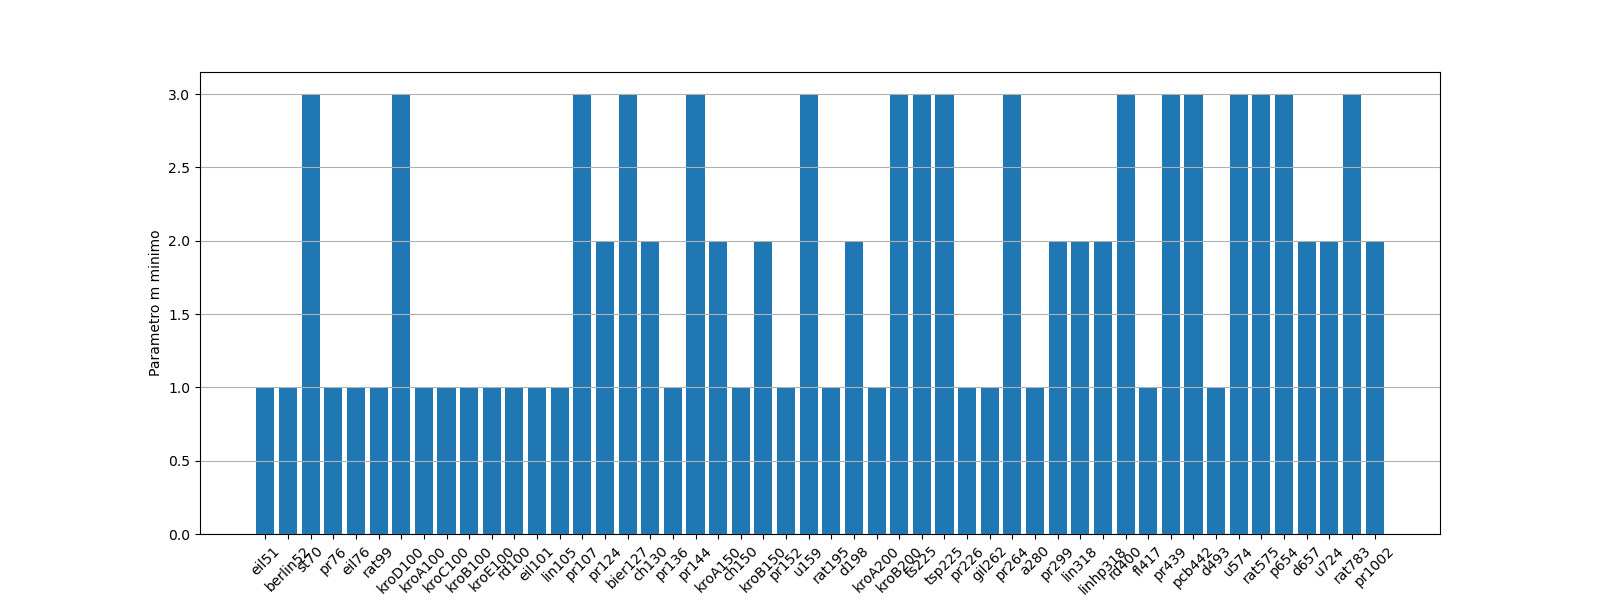
\includegraphics[width=1\textwidth]{../Grafici/1.png} \
In questo grafico a barre possiamo notare per ogni istanza (asse x, ordinati in base alla dimensione n) il parametro minimo m. Possiamo notare come tende a 1 per le istanze piccole (con alcune eccezioni) e tende a 3 per le istanze grandi (con migliaia di città).
\subsection{Analisi dei tempi delle versioni di Cheapest Insertion}
Una volta determinato il parametro minimo (e quindi il tempo minimo per quella versione), possiamo confrontare i tempi delle varie versioni per ogni istanza: \newline
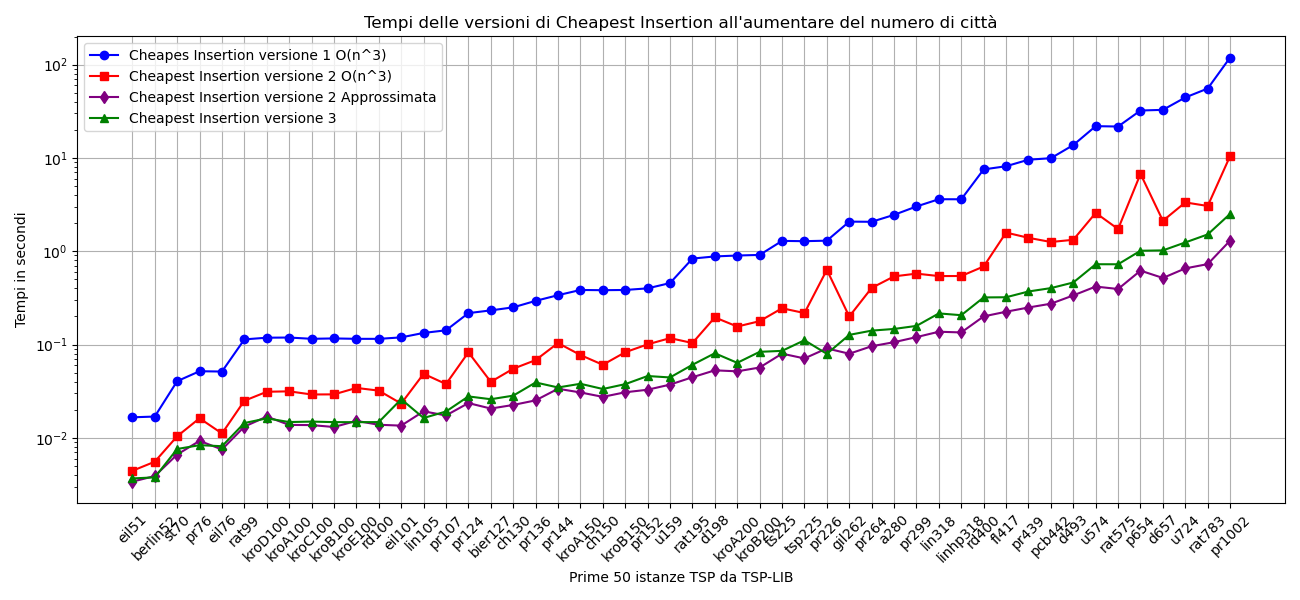
\includegraphics[width=1\textwidth]{../Grafici/2.png} \
In questo grafico possiamo notare come indubbiamente i tempi della prima versione $O(n^3)$ sono sempre peggiori delle altre versioni (compresa la seconda versione $O(n^3)$ anche se hanno stessa complessità temporale), allo stesso modo i tempi della seconda versione $O(n^3)$ è peggiore della terza versione $O(n^2 * m)$ (dove la m utilizzata per ottenere questi risultati è la m minima trovata precedentemente). Da un punto di vista dei tempi la l'implementazione migliore risulta essere la versione 2 approssimata, ovvero con complessità pari a $O(n^2)$, ma questa versione, come descritto nella sezione dedicata, non garantisce ad ogni iterazione di selezionare il nodo e il punto di inserzione ottimi, per questo motivo, dal punto di vista dei tempi, consideriamo la terza versione la migliore. Inoltre, aggiungo il fatto che il grafico mostra i tempi in scala logaritmica per una migliore leggibilità (i tempi variano da millesimi di secondo a centinaia di secondi).
\subsection{Analisi delle qualità delle versioni di Cheapest Insertion}
Dal punto di vista delle qualità trovate, le 3 versioni trovano in quasi tutti i casi lo stesso path e di conseguenza la stessa soluzione. Esistono però dei casi molto particolari nei quali, anche se l'algoritmo implementato è lo stesso, i path finali trovati sono diversi. Questo avviene perché ad ogni iterazione, l'implementazione deve determinare il nodo che, se inserito nel modo migliore possibile, ha costo di inserzione minimo, dopodiché procede ad inserire il nodo nel punto di inserimento ottimo. Il problema sorge nella misura in cui ad un determinato punto dell'esecuzione dell'euristica, sono presenti 2 punti di inserimento ottimi $(a_1, b_1)$ e $(a_2, b_2)$ per il nodo da inserire $v$ tali che $c_{a1v} + c_{vb1} - c_{a1b1} = c_{a2v} + c_{vb2} - c_{a2b2}$. Pertanto in presenza di un caso del genere, la scelta del punto di inserzione tra $(a_1, b_1)$ e $(a_2, b_2)$ è arbitrario, ma alla fine producono due path completamente diversi (con costi diversi). Per questo motivo il grafico sulle qualità delle soluzioni trovate dalle versioni è il seguente: \newline
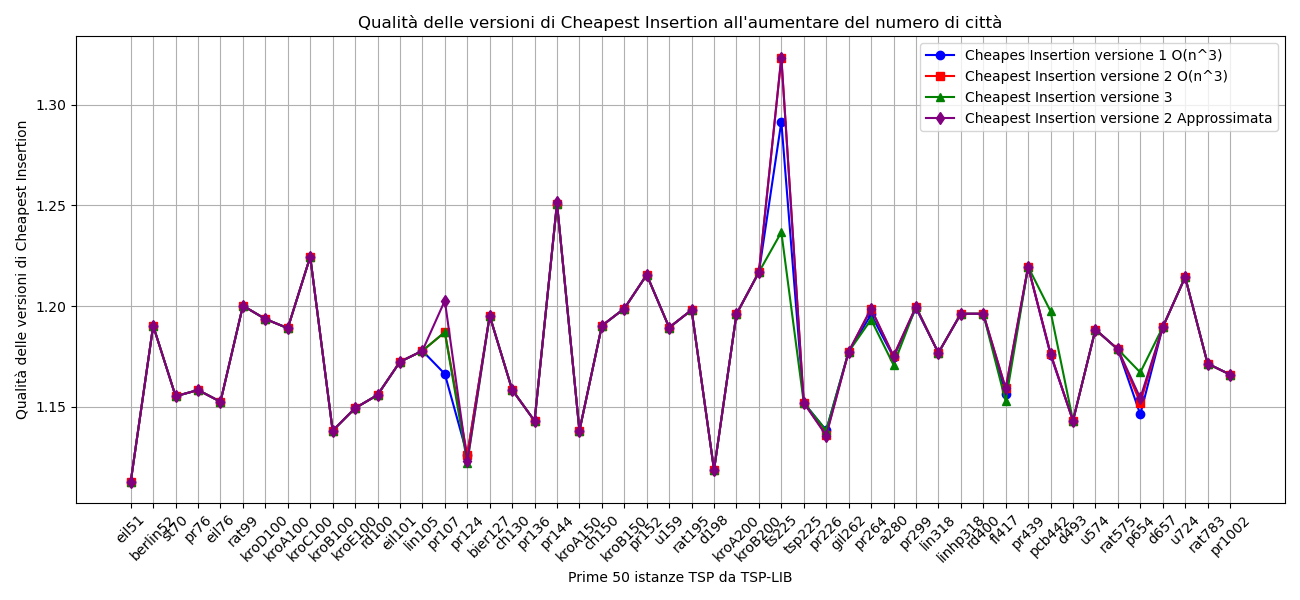
\includegraphics[width=1\textwidth]{../Grafici/3.png} \
In questo grafico possiamo notare come in quasi tutti i casi, le quattro varianti trovano gli stessi risultati, con alcune eccezioni: la versione approssimata non garantisce di selezionare il punto di inserzione ottimo (in quanto cerca solo "localmente" come visto in precedenza) e le versioni 2 e 3 a volte possono portare a soluzioni completamente diverse, anche se implementano correttamente l'euristica. Dati i risultati (sostanzialmente equivalenti) e date le grandi differenze di tempo viste nella sezione precedente, possiamo affermare che la terza versione sia complessivamente la migliore e sarà scelta come confronto con le altre euristiche.

\section{Confronto versioni Furthest Insertion}
In modo analogo alla sezione precedente, analizziamo prima di tutto la dimensione minima degli heap dei nodi fuori dal tour (versione 3) e procediamo poi a confrontare tempi e qualità.
\subsection{Dimensione ottimale degli heap per la versione 3 }
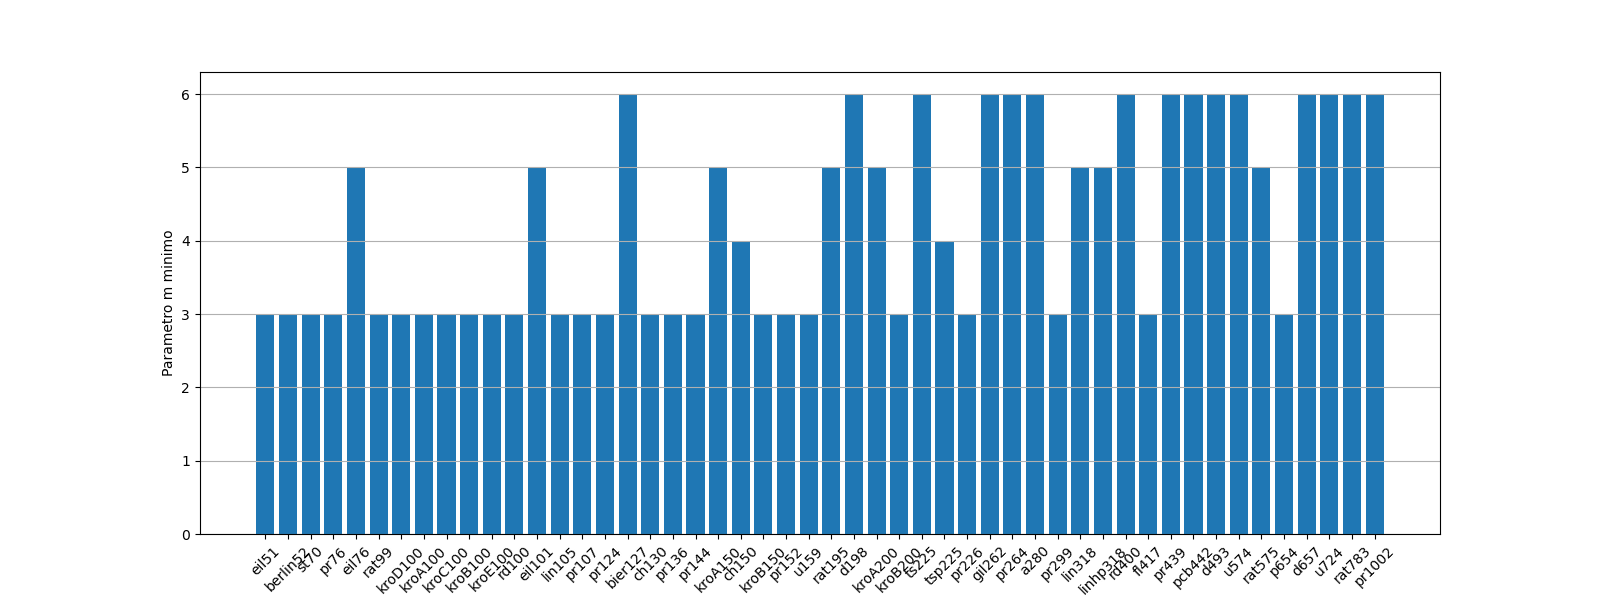
\includegraphics[width=1\textwidth]{../Grafici/4.png} \
Da questo grafico possiamo notare una importante differenza: la dimensione minima del parametro m è maggiore nel caso di Furthest Insertion rispetto a Cheapest Insertion: necessita sempre di un parametro m almeno pari a 3 fino alla dimensione massima pari a 6 (ci siamo limitati per questioni di tempo alle prime 50 istanze presenti su TSP-LIB). Per ogni istanza, l'implementazione ottimizzata userà la dimensione m minima trovata nelle successive analisi (come visto prima per Cheapest Insertion).
\subsection{Analisi dei tempi delle versioni di Furthest Insertion}
Di seguito il grafico dei tempi delle versioni di Furthest Insertion: \newline
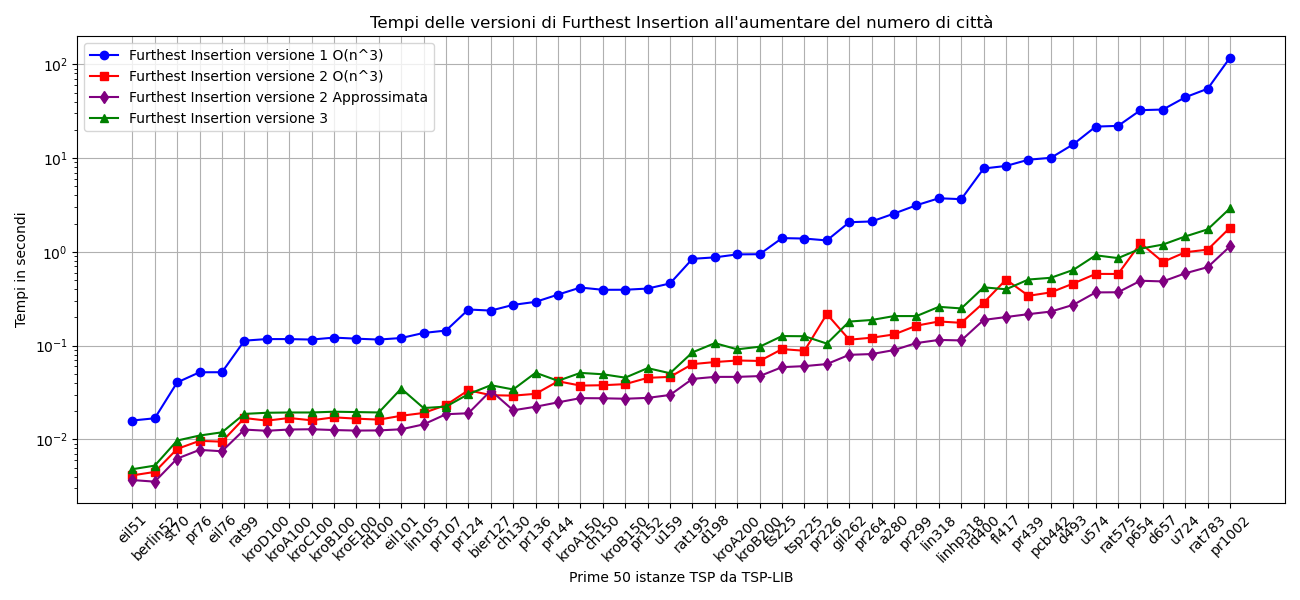
\includegraphics[width=1\textwidth]{../Grafici/5.png} \
Anche in questo caso è stato deciso di mostrare i dati con una scala logaritmica. Possiamo notare come la prima versione ($O(n^3)$ senza ottimizzazioni) risulta essere molto peggiore (in termini di tempo) rispetto alle altre versioni, inoltre questa differenza risulta essere più marcata rispetto a Cheapest Insertion versione 1. La versione 2 approssimata risulta essere la migliore in quanto ha complessità pari a $O(n^2)$ ma non la consideriamo in quanto non garantisce la scelta del nodo con costo di inserimento massimo (se inserito nel modo migliore possibile). Invece per quanto riguarda il confronto tra la versione 2 $O(n^3)$ e la versione ottimizzata $O(n^2 * m)$ risulta essere migliore la prima. Questo risultato può essere spiegabile con la seguente osservazione: effettuando un conteggio delle volte in cui la condizione if risulta vera (la condizione if che porta al terzo ciclo interno che rende la seconda versione $O(n^3)$) ci si rende conto che è vera in poche circostanze in contrasto con Cheapest Insertion versione 2 dove risultava vera molte volte, ad esempio:
\begin{myverbatim}
u1817: Cheapest -> 147917; Furthest -> 18993
u2319: Cheapest -> 112479; Furthest -> 25774
\end{myverbatim}
Questi sono i conteggi relativi al numero di volte che la condizione if (prima del terzo ciclo interno) risulti vera con la stessa istanza. Possiamo notare che nel caso di Furthest risulta essere un numero molto minore rispetto a Cheapest, per questo possiamo notare un miglioramento notevole dei tempi con l'ottimizzazione (dalla versione 2 alla 3 di Cheapest Insertion) mentre non notiamo questo miglioramento nel caso di Furthest Insertion.
\subsection{Analisi delle qualità delle versioni di Furthest Insertion}
Di seguito il grafico relativo alle qualità trovate dalle versioni di Furthest Insertion: \newline
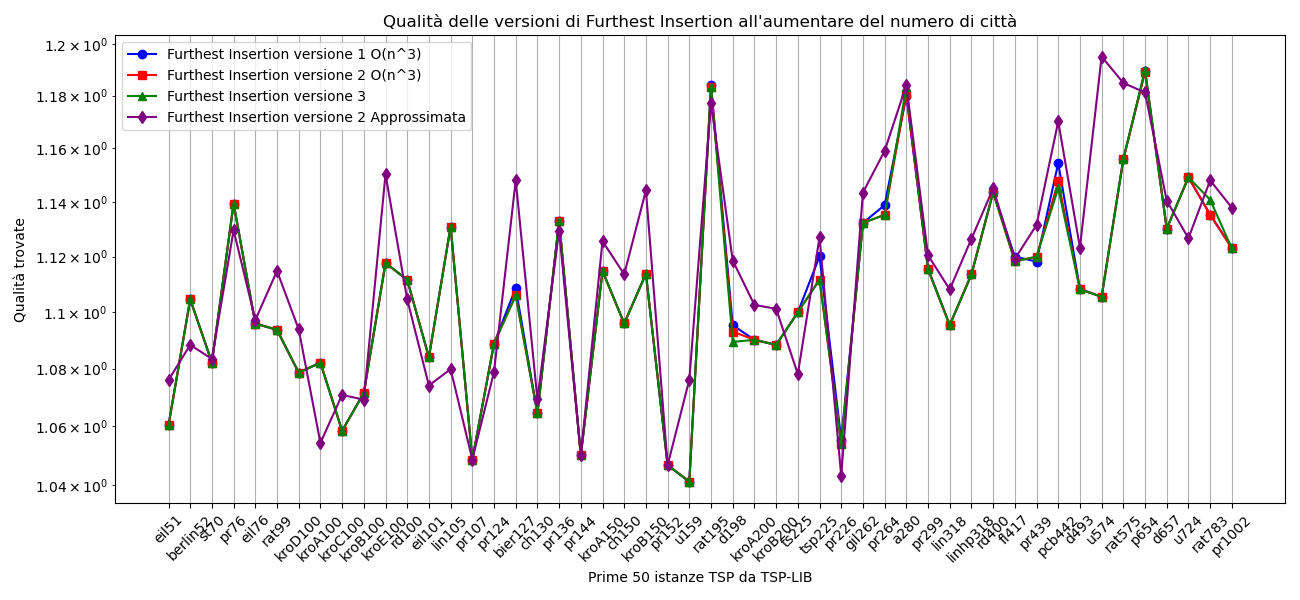
\includegraphics[width=1\textwidth]{../Grafici/6.png} \
In questo caso possiamo notare che la versione approssimata trova soluzioni molto diverse rispetto alle altre 3 euristiche in quanto non garantisce la scelta del punto di inserzione con costo di inserimento minimo. Inoltre notiamo la stessa differenza nelle altre euristiche discussa nella sezione precedente: la versione 1, 2 e 3 implementano correttamente l'euristica ma presentano risultati diversi in quanto sono presenti più punti di inserzione ottimo per lo stesso nodo. Di seguito lo stesso grafico senza la versione approssimata: \newline
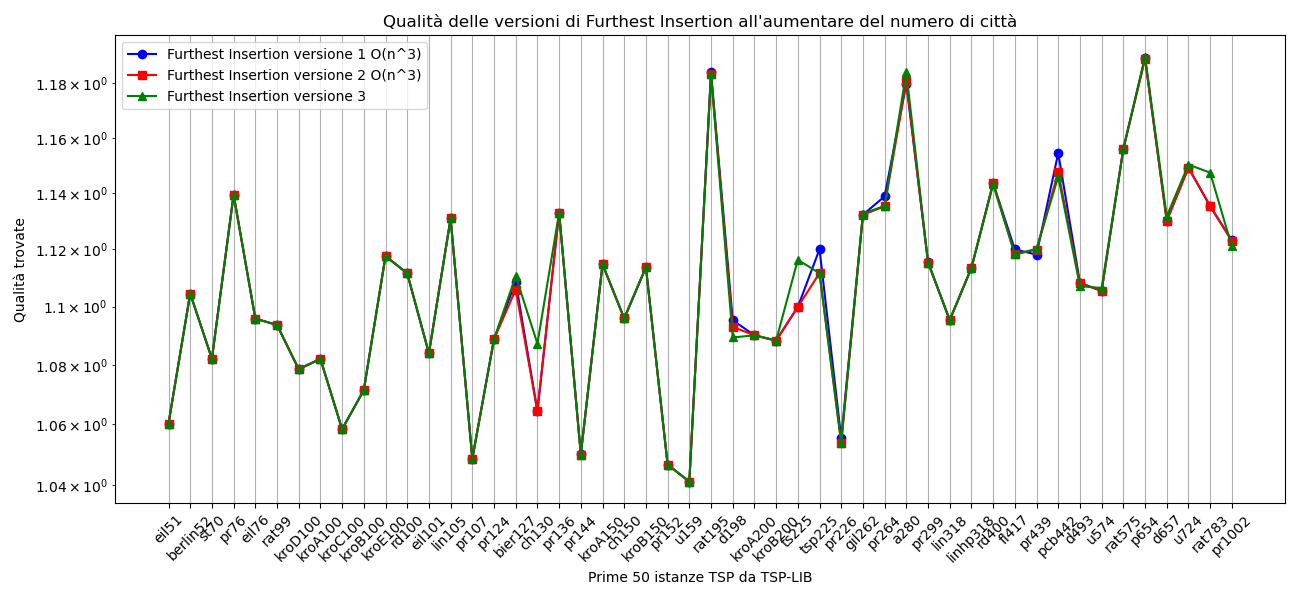
\includegraphics[width=1\textwidth]{../Grafici/6_2.png} \
In questo grafico possiamo notare come sono limitati i casi in cui le soluzioni trovate dalle 3 versioni sono diverse. \newline
Possiamo quindi concludere che la versione migliore (soprattutto dal punto di vista dei tempi in quanto le qualità delle soluzioni sostanzialmente si equivalgono) è la versione 2 e non la versione 3, ovvero la versione con un solo heap e non la versione con più heap per ogni nodo fuori dal tour.
\section{Confronto tempi e qualità delle euristiche}
In questo capitolo andremo a confrontare i risultati delle euristiche implementate nel capitolo precedente. Le euristiche che considereremo sono quindi:
\begin{legal}
  \item Nearest Neighbor
  \item Nearest Insertion
  \item Cheapest Insertion versione 3
  \item Farthest Insertion
  \item Furthest Insertion versione 2
\end{legal}
A differenza della sezione precedente, oltre ai tempi in questo caso le qualità trovate sono fondamentali nella valutazione delle euristiche. Ci limitiamo alla versione 3 di Cheapest Insertion versione 3 e Furthest Insertion versione 2 come visto nella sezione precedente. In questo caso analizzeremo qualità e tempi, ma sopratutto valuteremo anche le prestazioni su istanze enormi ($> 10000$ città). L'analisi delle versioni di randomInsertion e la robustezza delle euristiche riguardo l'inizializzazione sarà analizzata nei prossimi capitoli. Analizzeremo anche Nearest Neighbour anche se non è una euristica basata su inserzione per completezza.
\subsection{Analisi delle qualità delle euristiche}
Di seguito il grafico che mostra le qualità trovate dalle euristiche (asse y) per le prime 50 istanze presenti in TSP-LIB ordinate per numero di città (asse x): \newline
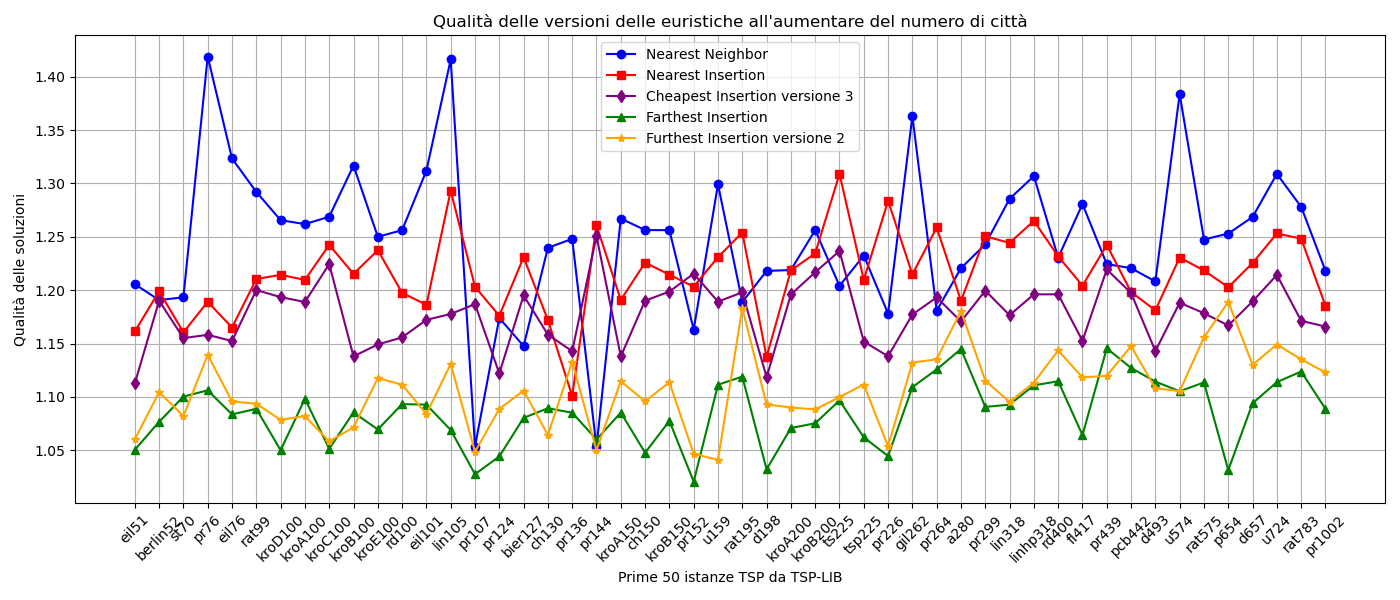
\includegraphics[width=1\textwidth]{../Grafici/7.png} \
Premettendo che si vuole una qualità più vicina possibile a 1 (quindi un costo totale più vicino possibile a quello ottimo), da questo grafico possiamo notare più cose: innanzitutto Nearest Neighbor risulta essere in molti contesti l'euristica peggiore, ad esempio per quanto riguarda le prime 10 città (a sinistra) risulta essere molto in alto rispetto alle altre soluzioni trovate (quindi ha trovato soluzioni peggiori), inoltre vale lo stesso discorso per molte istanze grandi verso le migliaia di città (a destra nel grafico). Il discorso analogo ma invertito vale per Furthest Insertion (ovvero l'euristica nuova proposta in questa tesi): possiamo notare come le qualità trovate sia per istanze piccole che grandi sia molte volte la migliore, con soluzioni trovate nella fascia tra il 10\% e il 20\% peggiori rispetto all'ottimo. Questo risultato è molto interessante confrontato con le altre euristiche che sembrano restare nella fascia 15\%-25\%. Possiamo effettuare una media delle soluzioni trovate, ottenendo:
\begin{myverbatim}
Nearest Neighbor ->              1.2470046772916366
Nearest Insertion ->             1.2156950870353294
Cheapest Insertion versione 3 -> 1.1782082768488287
Farthest Insertion ->            1.1910399037033677
Furthest Insertion versione 2 -> 1.1066458949521236
\end{myverbatim}
Ovvero in media (per le prime 50 città più piccole presenti su TSP-LIB) Furthest Insertion ottiene soluzioni di qualità significativamente superiore rispetto alle altre euristiche basate su inserzione (e anche rispetto a Nearest Neighbor). Questo risultato è particolarmente rilevante in quanto Furthest Insertion è proprio l'euristica mancante in letteratura. Per completezza possiamo anche valutare la varianza delle soluzioni trovate:
\begin{myverbatim}
Nearest Neighbor ->              0.0049800335629691375
Nearest Insertion ->             0.0014584496204975638
Cheapest Insertion versione 3 -> 0.0008967612647899936
Farthest Insertion ->            0.0023611070924068247
Furthest Insertion versione 2 -> 0.0012113120333807825
\end{myverbatim}
Da questi risultati possiamo concludere che Furthest Insertion trova soluzioni con una varianza tra le più basse (Cheapest Insertion ha una varianza più bassa). L'elevata varianza di Nearest Neighbor può essere spiegata anche graficamente: si possono notare qualità molto elevate (attorno al 40\%) e anche molto basse (attorno al 5\%).
\subsection{Analisi dei tempi delle euristiche}
Possiamo allo stesso modo analizzare i tempi delle euristiche analizzate nella sezione precedente: \newline
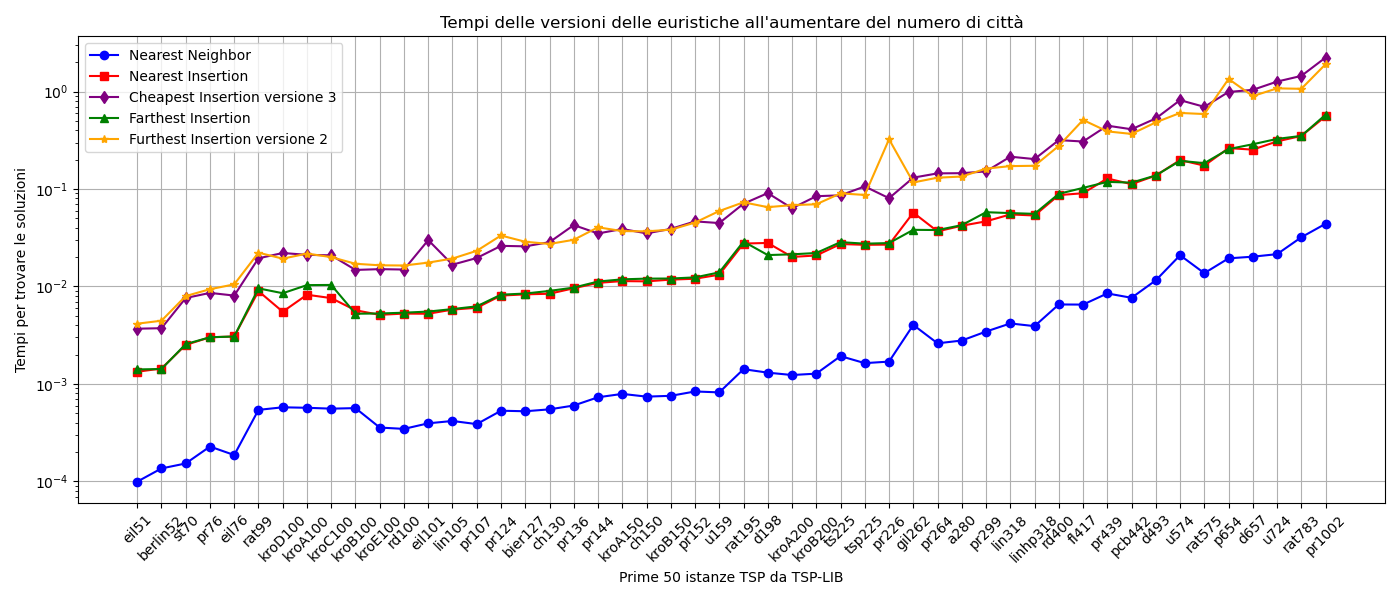
\includegraphics[width=1\textwidth]{../Grafici/8.png} \
I tempi sono coerenti con le considerazioni sulle complessità temporale fatte in precedenza: Nearest Neighbor risulta essere l'algoritmo più veloce con complessità $O(n^2)$ ma come visto in precedenza in media trova soluzioni di qualità bassa, Nearest Insertion e Farthest Insertion hanno un tempo molto simile in quanto entrambi sono algoritmi $O(n^2)$ e condividono molto del codice, mentre Cheapest Insertion e Furthest Insertion anche in questo caso ottengono tempi molto simili e coerenti con la loro complessità temporale (analizzata nelle sezioni precedenti). \newline Complessivamente (in sintesi) possiamo affermare che Furthest Insertion trova in media le soluzioni migliori ma richiede più tempo rispetto alle altre euristiche (tranne nel caso di Cheapest Insertion dove i tempi sono molto simili).

\section{Confronto tempi e qualità delle euristiche con istanze enormi}
In questa sezione analizziamo il comportamento delle euristiche nel caso di istanze molto grandi (con un numero di città maggiore uguale a 10000), per motivi di tempo saranno analizzate un numero limitato di queste istanze enormi ovvero le istanze: rl11849, usa13509, brd14051, d15112, d18512. Per prima cosa è necessario ottenere il parametro m minimo per queste istanze per Cheapest Insertion versione 3, le dimensioni minime trovate sono:
\begin{myverbatim}
DA COMPLETARE
\end{myverbatim}

\section{Analisi robustezza delle implementazioni rispetto alla scelta delle città iniziali}
Abbiamo visto che l'inizializzazione del tour consiste nel determinare la coppia di città più vicine per gli algoritmi Nearest Neighbor, Nearest Insertion e Cheapest Insertion e consiste nel determinare la coppia di città più lontane per Farthest e Furthest Insertion. Questa sezione analizza il variare dei tempi e delle qualità delle soluzioni trovate al variare delle città iniziali. Per fare questo (come visto nella sezione delle implementazioni) l'implementazione resta la stessa tranne per il fatto che le due città iniziali sono scelte casualmente. Chiaramente si deve garantire che siano due città diverse. Vediamo i risultati prima dal punto di vista delle qualità, poi dei tempi.
\subsection{Robustezza della qualità della soluzione delle implementazioni}
Per prima cosa valutiamo la robustezza della qualità della soluzione, quindi iteriamo 100 volte (con un seed diverso per i numeri casuali) sulle prime 30 istanze da TSP-LIB in ordine di dimensione, ho deciso di limitarmi alle sole prime 30 città in quanto iterare 100 volte sull'esecuzione di tutte e 5 le euristiche richiede molto tempo. Per prima cosa considero la media delle soluzioni trovate per ogni istanza e per ogni algoritmo: \newline
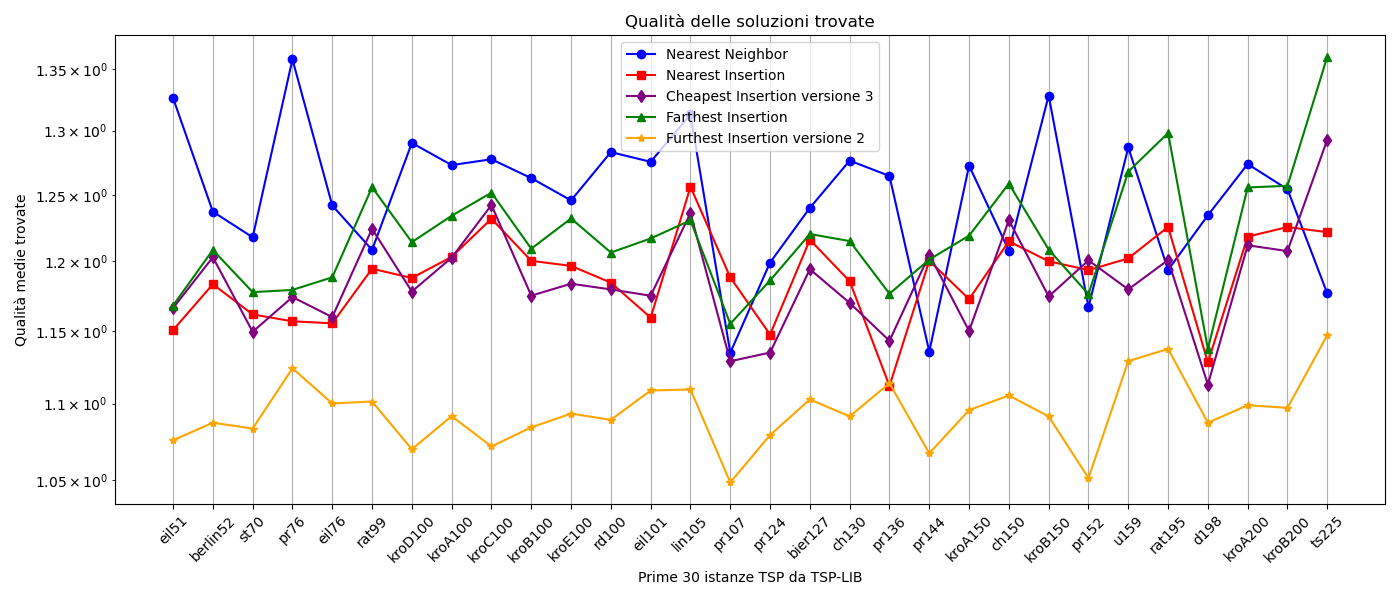
\includegraphics[width=1\textwidth]{../Grafici/9.png} \
I risultati medi sono coerenti con i risultati ottenuti inizializzando il tour con la coppia di città più vicine/lontane: Furthest Insertion (nelle 30 città analizzate) trova sempre un percorso migliore rispetto alle altre euristiche analizzate, trovando soluzioni tra 5\% e il 15\%, mentre le altre euristiche si collocano nel range 10\%-25\% (o 30\% nel caso di Nearest Neighbour). Inoltre in particolare Nearest Neighbor trova soluzioni (in media) peggiori rispetto alle altre euristiche. \newline 
Ora possiamo analizzare invece la varianza delle soluzioni trovate: vogliamo quindi sapere quanto le soluzioni sia llontanano dal valore medio trovato prima al variare dell'inizializzazione. Di seguito il grafico: \newline
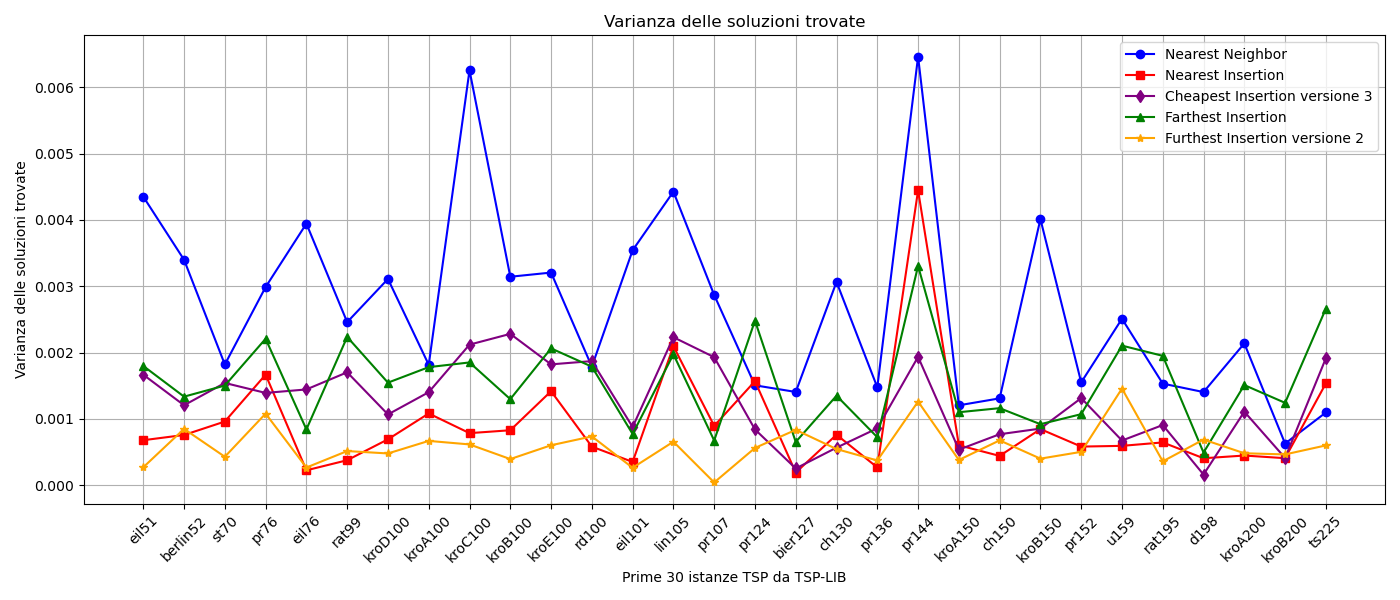
\includegraphics[width=1\textwidth]{../Grafici/10.png} \
Possiamo notare come Nearest Neighbor ha una varianza elevata, quindi le soluzioni trovate distano molto dalla media (avvicinandosi o allontanandosi dall'ottimo). Dopodiché possiamo notare come Furthest Insertion abbia una varianza tra le più basse (possiamo forse affermare che abbia la varianza più bassa), andando a considerare la media delle varianze otteniamo:
\begin{myverbatim}
Nearest Neighbor ->              0.002681760251702191
Nearest Insertion ->             0.0009059930614140123
Cheapest Insertion versione 3 -> 0.00125661452221978
Farthest Insertion ->            0.001547882691714873
Furthest Insertion versione 2 -> 0.0005832323004466427
\end{myverbatim}
Da questi risultati possiamo notare come Furthest Insertion abbia la varianza più bassa tra le euristiche analizzate: questo è un altro risultato interessante, ovvero non solo trova (in media) le soluzioni più vicine all'ottimo (con inizializzazione casuale e non) ma anche con una varianza bassa.
\subsection{Robustezza dei tempi delle implementazioni}
In questa sezione vogliamo invece vedere come variano i tempi delle implementazioni sempre con una inizializzazione casuale del tour. Come prima, innanzitutto analizziamo la media dei tempi e poi la varianza. \newline
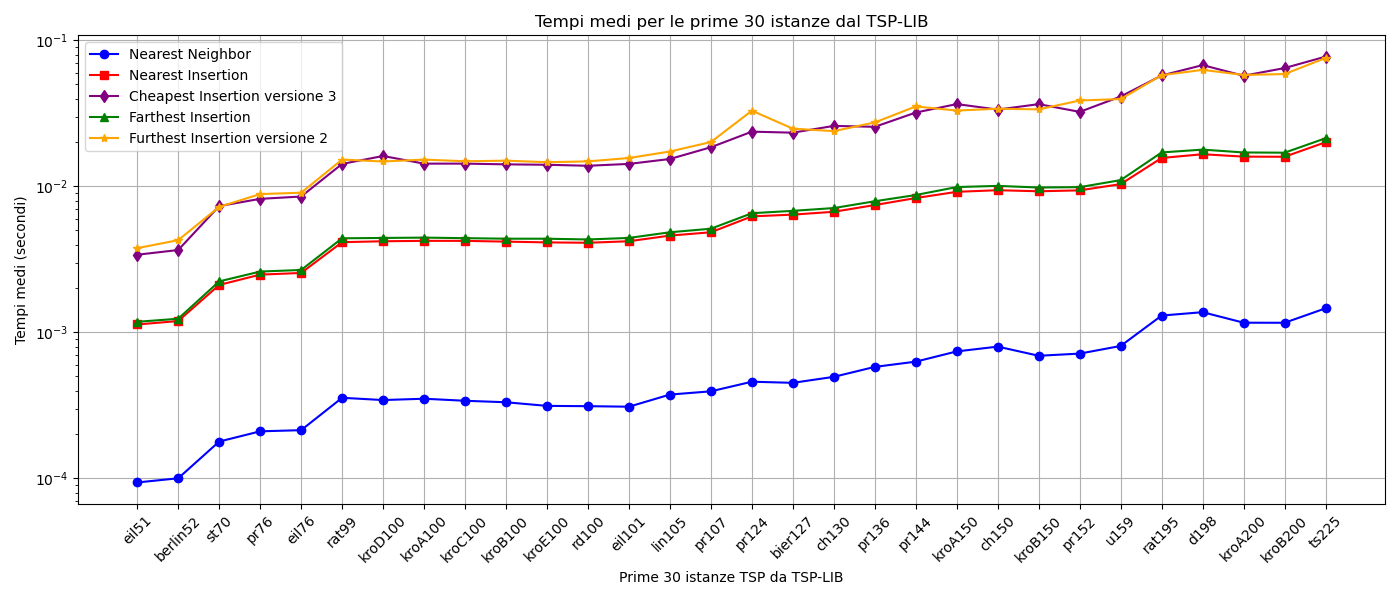
\includegraphics[width=1\textwidth]{../Grafici/11.png} \
Anche in questo caso, i risultati non si allontano molto dai risultati ottenuti con l'inizializzazione delle città più vicine/lontane: Nearest Neighbor si conferma come euristica più veloce, dopodiché Nearest Insertion e Farthest Insertion ottengono tempi medi molto simili e infine Cheapest Insertion e Furthest Insertion ottengono tempi medi molto simili (i peggiori in modo coerente con la complessità temporale).  \newline
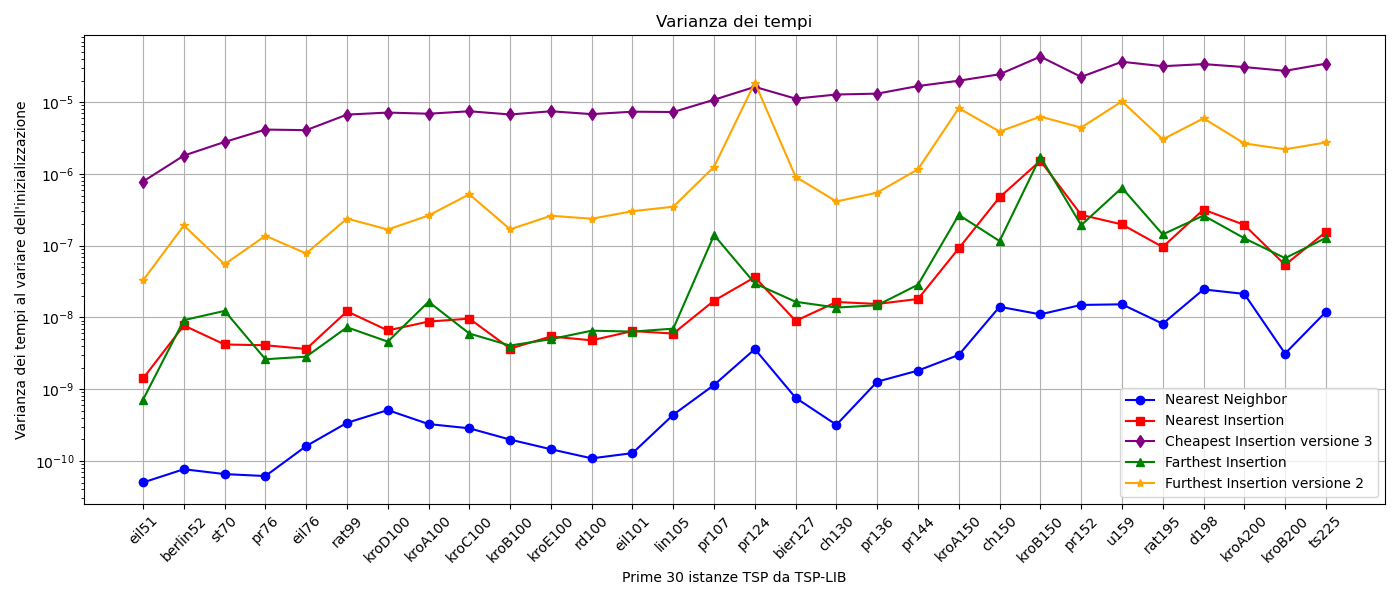
\includegraphics[width=1\textwidth]{../Grafici/12.png} \
Dal punto di vista invece della varianza dei tempi, possiamo notare una varianza molto bassa per i tempi per Nearest Neighbor, dopo (in ordine) una varianza bassa per Nearest Insertion e Farthest Insertion, poi Furthest Insertion con una varianza relativamente alta e infine Cheapest Insertion versione 3 con la varianza più alta per quanto riguarda i tempi.


 
%
%			BIBLIOGRAFIA
%

\begin{thebibliography}{00}
\bibitem{Menger}
Traveling Salesman Problem, F. Greco, IntechOpen, 2008.
\bibitem{TSP formulation}
M. Velednitsky, Short Combinatorial Proof that the DFJ Polytope is contained in
the MTZ Polytope for the Asymmetric Traveling Salesman Problem, UC Berkeley, 2018.
%
\bibitem{Analysis of Brute Force}
Analysis of Brute Force and Branch \& Bound Algorithms to solve the Traveling
Salesperson Problem (TSP), Informatics Department, Engineering Faculty, Widyatama University, 2021.
%
\bibitem{Branch and Bound}
T. G. Crainic, B. Le Cun, C. Roucairol, Parallel Branch-and-Bound Algorithms, Département de management et technologie École des Sciences de la Gestion Université du Québec à Montréal and CIRRELT, Canada
\bibitem{Branch and Cut Algoritmhs}
Yuan Yuan, Diego Cattaruzza, Maxime Ogier, Frederic Semet. A branch-and-cut algorithm for the generalized traveling salesman problem with time windows. European Journal of Operational Research, 2020, 286 (3)
%
\bibitem{TSP NP Completezza}
R. Karp, Complexity of the Traveling Salesman Problem
%
\bibitem{Reinelt}
G. Reinelt, The Traveling Salesman: Computational Solution for TSP Applications, Heidelberg, Springer-Verlag
\bibitem{Branch and Cut}
J.E. Mitchell, Branch-and-cut algorithms for combinatorial
optimization problems, in Handbook of applied optimization, P.M.
Pardalos and M.G.C. Resende eds., Oxford University Press, 2000
\bibitem{Local Search}
Olaf Mersmann, Bernd Bischl, Jakob Bossek, Heike Trautmann, Markus Wagner, Frank Neumann, Local Search and the Traveling Salesman Problem: A Feature-Based Characterization of Problem Hardness, Statistics Faculty, TU Dortmund University, Germany
\bibitem{2OPT}
Matthias Englert, Heiko Röglin, Berthold Vöcking, Worst Case and Probabilistic Analysis 
of the 2-Opt Algorithm for the TSP, Dept. of Computer Science, RWTH Aachen University
\bibitem{LK}
S. Lin, B. W. Kernighan, An Effective Heuristic Algorithm for the Traveling-
Salesman Problem, Bell Telephone Laboratories, Incorporated, Murray Hill, N.J., 1971
\bibitem{Helsgaun}
K. Helsgaun, An effective implementation of the Lin-Kernighan traveling
salesman heuristic, Department of Computer Science, Roskilde Universit, 13 April 1999
\bibitem{knuthart}
Donald E. Knuth, The Art of Computer Programming: Volume 2 (Seminumerical Algorithms),Addison-Wesley Professional, 1997, Capitolo 3


%\bibitem{gotti91}
%M. Gotti, I linguaggi specialistici, Firenze, La Nuova Italia, 1991.
\end{thebibliography}
% 
\end{document}


 
